\documentclass[10pt,twocolumn]{article}

% ---- packages ----
\usepackage[utf8]{inputenc}
\usepackage[T1]{fontenc}
\usepackage{lmodern}
\usepackage[margin=0.75in]{geometry}
\usepackage{microtype}
\usepackage{amsmath,amssymb}
\usepackage{graphicx}
\usepackage{booktabs}
\usepackage{array}
\usepackage{multirow}
\usepackage{xcolor}
\usepackage{hyperref}
\usepackage{url}
\usepackage{enumitem}
\usepackage{titlesec}
\usepackage{caption}
\usepackage{float}
\usepackage[numbers,sort&compress]{natbib}

\hypersetup{
  colorlinks=true,
  linkcolor=blue!55!black,
  citecolor=green!45!black,
  urlcolor=blue!70!black,
}

\graphicspath{{figures/}}
\setlength{\parskip}{0.25em}
\titlespacing*{\section}{0pt}{1.1em}{0.5em}
\titlespacing*{\subsection}{0pt}{0.8em}{0.35em}

% convenience macros
\newcommand{\aep}{AEP}
\newcommand{\ajo}{AJO}
\newcommand{\todo}[1]{\textcolor{red}{[TODO: #1]}}

\title{\textbf{Causal Embedding Models for Procedural Documentation:\\
A Survey of Methods for Follow-up Reranking and Workflow Ordering}}

\author{Causal Embedding Research \\ \texttt{Adobe Experience Platform / Journey Optimizer}}
\date{\today}

\begin{document}
\maketitle

\begin{abstract}
We study the design of \emph{causal embedding models}: representations and scoring
functions that capture the \emph{directional, precedence} structure of procedural
documentation rather than mere topical similarity. Our concrete setting is the
documentation and video tutorials of Adobe Experience Platform (\aep) and Adobe
Journey Optimizer (\ajo), from which a model must (i) judge whether one step
\emph{causally precedes / enables} another, (ii) \textbf{rerank candidate follow-up
questions} by logical progression, and (iii) \textbf{sort multi-step workflows into
ascending order}. We survey the landscape end to end---causal representation learning
and causal reasoning from text; the state of the art in dense retrieval and
bi-/cross-/late-interaction architectures; \emph{asymmetric and order-structured
embedding geometries} (order, box, Gaussian, and hyperbolic/Lorentz embeddings) that
natively express directionality; reasoning rerankers and reinforcement learning for
ranking in sub-1B models; sentence/step ordering and robust rank aggregation; and
follow-up/conversational retrieval and procedural-workflow understanding. We ground the
survey in an empirical characterization of the project's own data and baselines---where
a bi-encoder wins pairwise classification but a DeBERTa cross-encoder wins workflow
ordering (21/30 vs.\ 0/30), exposing that \emph{pairwise accuracy $\neq$ ordering
quality}. We argue that the dominant failure mode is not the pairwise model but the
\emph{aggregation} (naive topological sort collapses on a single cycle) and the
\emph{data} (adjacent-only, total-order labels). We synthesize a concrete, sub-1B system
design---calibrated cross-encoder $\rightarrow$ minimum-feedback-arc-set / Kemeny
aggregation $\rightarrow$ partial-order evaluation, with distilled ``think-free'' causal
rationales and an optional ordering-reward GRPO polish---and release a reference
implementation of the aggregation, calibration, metrics, and reranking components.

\end{abstract}

\section{Introduction}

\subsection{Motivation}
Enterprise documentation is overwhelmingly \emph{procedural}: it tells a user how to
accomplish a goal through an ordered sequence of steps. Adobe Experience Platform
(\aep) and Adobe Journey Optimizer (\ajo) ship thousands of documentation pages and
video tutorials describing how to build audiences, enrich profiles, design journeys, and
orchestrate campaigns. A retrieval or assistant system over this corpus must do more than
return topically similar passages---it must understand \emph{what comes before what}.
Concretely, three downstream capabilities motivate this survey:

\begin{enumerate}[leftmargin=1.4em,itemsep=0.15em]
  \item \textbf{Directional causal judgment.} Given two pieces of text
  (steps, phases, or doc fragments) $t_1$ and $t_2$, estimate
  $P(t_1 \text{ causally precedes / enables } t_2)$.
  \item \textbf{Follow-up question reranking.} Given a user question, order a slate of
  candidate follow-up questions by logical/causal progression, not just relevance.
  \item \textbf{Workflow ordering.} Given the unordered steps of a workflow, sort them
  into the correct ascending execution order.
\end{enumerate}

All three rest on a single primitive---a \emph{directional}, asymmetric notion of
precedence---that standard semantic embeddings, built around symmetric cosine
similarity, do not natively provide. We call a model that captures this primitive a
\emph{causal embedding model}, and we use the term deliberately broadly: it spans
asymmetric scoring heads over encoders, order/box/hyperbolic geometries, cross-encoder
reasoners, and small generative rerankers. The foundations section clarifies precisely
which rung of Pearl's causal ladder this task occupies (largely structural precedence,
not intervention).

\subsection{Why this is hard}
Three difficulties recur throughout the survey. First, \emph{symmetry}: the workhorse
similarity function $\cos(\mathbf{a},\mathbf{b})$ is symmetric, so a vanilla embedding
cannot, by construction, distinguish ``$A$ enables $B$'' from ``$B$ enables $A$.''
Second, \emph{causal direction is genuinely hard}: even frontier LLMs perform poorly on
pure causal-direction benchmarks, and supervised systems cap well below ceiling. Third,
and most consequentially for us, \emph{local correctness does not compose into global
correctness}: a model can be accurate on most individual pairs yet still produce a wholly
wrong global order, because the step that turns $O(n^2)$ noisy pairwise judgments into a
single ranking is fragile. In this project, a DeBERTa-v3 cross-encoder that orders a
6-step workflow nearly correctly and scores 21/30 on pairwise direction nonetheless
yields \textbf{0/30} correct \emph{full orderings} under a naive topological sort---a
gap this survey takes as its central diagnostic.

\subsection{Scope and contributions}
This document is both a \emph{survey} and a \emph{system-design study} grounded in a
real, ongoing project under a strict \textbf{sub-1B-parameter} budget and a
4$\times$A100 environment. Our contributions are:

\begin{itemize}[leftmargin=1.4em,itemsep=0.15em]
  \item A structured survey of the methods relevant to causal/directional embeddings,
  spanning eight areas: causal foundations, embedding/retrieval architectures, causal
  reasoning from text, asymmetric/order-structured geometry, reasoning rerankers and RL,
  sentence-ordering and rank aggregation, follow-up/conversational retrieval, and
  procedural-workflow understanding.
  \item An empirical characterization of the project's corpus, pairwise datasets, tier
  system, and follow-up data, with the baselines any new model must beat.
  \item A diagnosis that reframes the workflow-ordering failure as primarily an
  \emph{aggregation} and \emph{data} problem rather than a pairwise-model problem, and a
  concrete sub-1B system design that follows from it.
  \item A reference implementation (released alongside this survey) of robust ordering
  (minimum-feedback-arc-set, Bradley--Terry, Kemeny), score calibration, partial-order
  metrics, and a model-free follow-up reranker.
\end{itemize}

\subsection{Organization}
Section~2 establishes causal foundations and a working definition of ``causal
embedding.'' Section~3 surveys dense-retrieval architectures and modern embeddings.
Section~4 covers causal reasoning and direction from text. Section~5 develops asymmetric
and order-structured geometries---the most direct route to directionality. Section~6
surveys reasoning rerankers and RL for ranking under a small-model budget; Section~7
covers turning pairwise scores into a global order. Section~8 addresses follow-up and
conversational retrieval; Section~9, procedural-workflow understanding. Section~10
characterizes the data. Section~11 synthesizes a recommended system and roadmap, and
Section~12 concludes.

\section{Foundations: What Is a ``Causal'' Embedding?}
\label{sec:foundations}

The phrase ``causal embedding'' is used loosely across the retrieval and
representation-learning literature, often as a synonym for any embedding whose
geometry encodes \emph{asymmetric} relations. This section pins down what we
mean precisely, separates three distinct notions that are routinely conflated,
and locates the project's goal --- directional precedence between documentation
steps --- on the firmest defensible footing. We are deliberately conservative:
we argue that a ``causal embedding'' for procedural documentation is, in the
honest analysis, a model of \emph{structural / directional precedence learned
from text}, sitting almost entirely at the lowest rung of Pearl's ladder, and we
say so plainly rather than overclaiming interventional or counterfactual
content.

\subsection{Three notions routinely conflated}
\label{sec:three-notions}

\paragraph{(i) Statistical / semantic similarity.}
The default embedding objective --- contrastive or masked-language pretraining,
then a cosine/dot-product similarity --- produces a \emph{symmetric},
\emph{undirected} notion of relatedness: $\mathrm{sim}(a,b)=\mathrm{sim}(b,a)$.
Two documentation steps that mention the same dataset, schema, or UI panel land
near each other regardless of which must happen first. This is exactly the
shortcut our project must defeat: in the repo's hardest ordering dataset
(\texttt{ajo\_newstyle}), the best symmetric similarity model collapses to
$\approx 65\%$ accuracy because topical overlap and step order are decorrelated
on purpose. Semantic similarity is a \emph{necessary} substrate (it gives a
strong stage-1 retriever) but is provably insufficient for ordering: any
symmetric kernel assigns the pair $(A,B)$ and $(B,A)$ identical scores and
therefore carries zero bits about direction.

\paragraph{(ii) Asymmetric / directional relations.}
The next notion drops symmetry without yet claiming causality. Entailment is the
canonical example: ``$P$ entails $H$'' does not imply ``$H$ entails $P$''
\citep{found:bowman2015snli,found:williams2018mnli}. Order embeddings,
hyperbolic/entailment cones, and asymmetric dual encoders (a query tower and a
document tower with untied weights) all realize a scoring function
$s(a\!\to\!b)\neq s(b\!\to\!a)$. Temporal precedence (``$A$ occurs before $B$'')
and prerequisite structure also live here. Crucially, \emph{asymmetry is not
causality}: an asymmetric relation can encode narration order, set inclusion, or
specificity, none of which is a causal mechanism. Most so-called ``causal
embeddings'' in practice are this --- a learned directional relation --- and the
honest claim stops here.

\paragraph{(iii) Genuine causal structure.}
The strongest notion requires that the represented relation track an underlying
data-generating mechanism: $A\to B$ means intervening on $A$ changes the
distribution of $B$, while intervening on $B$ does not change $A$
\citep{found:pearl2009causality,found:peters2017elements}. This is defined with
respect to a structural causal model (SCM) and is identified, in the
observational regime, only under assumptions (Sec.~\ref{sec:direction-id}). For
text, we essentially never observe interventions on documentation steps, so
genuine causal structure is at best \emph{inferred} from the asymmetries the
text exposes. Our position: the project targets notion~(ii) as a tractable proxy
for notion~(iii), and the contribution is making that proxy as faithful as the
text allows.

\paragraph{Problem statement.}
Formally, given an ordered pair of texts $(t_1,t_2)$ we want a model
$f_\theta(t_1,t_2)\to[0,1]$ estimating $P(t_1 \text{ causally precedes /
enables } t_2)$, with the constraints (a) \emph{antisymmetry},
$f_\theta(t_1,t_2)\approx 1-f_\theta(t_2,t_1)$ for genuinely directional pairs,
and (b) an \emph{abstain / NEUTRAL} option for independent or parallel steps so
that the induced relation is a partial order (DAG), not a forced total order.
Downstream we need this primitive to (1) classify direction, (2) rerank
follow-ups, and (3) sort a workflow. A pure bi-encoder embedding cannot satisfy
(a) by construction unless direction is injected via untied towers or an
asymmetric scoring head; this motivates the cross-encoder / interaction-based
designs surveyed later.

\subsection{Causal representation learning: what it gives and does not give for text}
\label{sec:crl}

The modern program of \emph{causal representation learning} (CRL)
\citep{found:scholkopf2021causalrl} seeks to recover latent variables that
correspond to causal factors of variation and to learn the causal graph among
them, rather than entangled statistical features. Three pillars are relevant.

\paragraph{Independent causal mechanisms (ICM).}
The ICM principle holds that the causal generative process factorizes into
autonomous modules $P(X)=\prod_i P(X_i\mid \mathrm{pa}_i)$ whose mechanisms are
independent: changing one mechanism (an intervention) leaves the others
invariant \citep{found:peters2017elements,found:scholkopf2021causalrl}. This
\emph{invariance} is the deepest reason causal features generalize across
distribution shift, and it underlies invariant-risk and domain-generalization
objectives \citep{found:arjovsky2019irm,found:gulrajani2021domainbed}. For our
setting, ICM is aspirational: it suggests that a step's \emph{enabling
preconditions} should be an invariant module reusable across workflows, which is
precisely the generalization we need for far-apart (non-adjacent) step pairs.

\paragraph{Disentanglement and identifiability.}
A central negative result is that disentangled representations are
\emph{not identifiable} from i.i.d.\ observations without inductive biases or
weak supervision \citep{found:locatello2019challenging}: infinitely many latent
factorizations explain the same marginal. CRL therefore leans on auxiliary
signals --- multiple environments, interventions, temporal structure, or paired
data --- to pin down the causal factors \citep{found:scholkopf2021causalrl}.
\textbf{What this means for text:} we have no controlled interventions on
documentation, but we \emph{do} have weak supervision (the antisymmetric
forward/reverse labels, multiple documents, tier metadata). The identifiability
literature warns that direction learned from a single narration order is
under-determined --- it can latch onto narration rather than mechanism --- which
is exactly the failure diagnosed in the repo data (training only on adjacent,
same-document pairs teaches narration order, not causal necessity). CRL thus
does \emph{not} hand us a causal text embedding for free; it tells us which
auxiliary signals (non-adjacent pairs, multiple sources, abstention) are needed
to make direction identifiable.

\subsection{Pearl's ladder and where a documentation ``causal embedding'' sits}
\label{sec:ladder}

Pearl's \emph{ladder of causation} stratifies causal questions into three rungs
\citep{found:pearl2009causality,found:pearl2018book}:

\begin{description}[leftmargin=1.2em,itemsep=2pt]
  \item[Rung 1 --- Association] $P(y\mid x)$: ``seeing.'' Correlation,
  conditional probability, similarity. All standard embeddings live here.
  \item[Rung 2 --- Intervention] $P(y\mid \mathrm{do}(x))$: ``doing.'' The effect
  of actively setting $x$, requiring an SCM or experiments.
  \item[Rung 3 --- Counterfactual] $P(y_x\mid x',y')$: ``imagining.'' What would
  have happened had $x$ been different, holding the realized world fixed.
\end{description}

\noindent\textbf{An honest placement.}
A causal embedding for procedural documentation operates predominantly at
\emph{Rung 1 with structural / directional precedence layered on top}. We are
estimating an associational quantity --- $P(\text{$t_1$ precedes $t_2$}\mid
t_1,t_2)$ --- that we \emph{interpret} as enablement. We are not running
$\mathrm{do}(\cdot)$ on a workflow, and we are not computing counterfactual
re-orderings of a tutorial. The directional supervision (forward/reverse labels)
nudges the representation toward the asymmetry that a Rung-2 mechanism would
induce, but the trained object remains a Rung-1 estimator of a directed relation.
This is the single most important caveat in the survey: claiming Rung-2/3
content for a text embedding trained on observational documentation would be an
overclaim. Where genuine intervention-style evidence exists in our data, it is
implicit (``you cannot publish before you authenticate'' is a logical/temporal
precondition recoverable from text, not an experiment).

\subsection{Causal direction identification (background, then pivot to text)}
\label{sec:direction-id}

Outside NLP, the \emph{bivariate} causal-direction problem --- given samples of
$(X,Y)$, decide $X\to Y$ vs.\ $Y\to X$ --- is the cleanest analog of our pairwise
task. Because the joint $P(X,Y)$ is symmetric, direction is identifiable only
under structural assumptions that break the symmetry:

\begin{itemize}[leftmargin=1.2em,itemsep=2pt]
  \item \textbf{Additive Noise Models (ANM)} \citep{found:hoyer2008anm}:
  assume $Y=f(X)+N$, $N\!\perp\!X$. A nonlinear $f$ typically admits an
  independent-noise fit in only one direction; one regresses both ways and tests
  residual independence (HSIC) to pick the direction with independent residuals.
  \item \textbf{LiNGAM} \citep{found:shimizu2006lingam}: linear non-Gaussian
  acyclic models identify direction via independent-component analysis on the
  non-Gaussian noise.
  \item \textbf{IGCI} \citep{found:janzing2012igci}: information-geometric causal
  inference assumes independence between the cause distribution and the
  mechanism, scoring an asymmetry in their ``alignment.''
\end{itemize}

\noindent The standard testbed is the \emph{T\"ubingen cause-effect pairs}
benchmark of $\approx 100$ expert-labeled real bivariate pairs
\citep{found:mooij2016distinguishing}; reported accuracies cluster around
$\sim$60--72\% for IGCI/ANM-style methods --- i.e.\ direction is hard even with
clean numeric data and explicit modeling assumptions. \textbf{The pivot to
text:} documentation gives us neither i.i.d.\ numeric samples nor a clean noise
model. Instead, the asymmetry-revealing signal is \emph{linguistic} ---
discourse connectives, temporal markers, prerequisite phrasing, and world
knowledge --- which is why the rest of this survey treats causal direction in
text as a supervised pairwise classification / entailment problem
(Sec.~\ref{sec:causal-reasoning}) rather than an ANM/IGCI estimation problem.
The bivariate literature contributes the conceptual lesson, not the algorithm:
direction must come from an assumption or supervision that breaks the symmetry of
$P(X,Y)$, and for text that assumption is encoded in the antisymmetric labels and
the cross-attention architecture.

\subsection{A taxonomy of ``causal'' embeddings}
\label{sec:taxonomy}

Table~\ref{tab:found-taxonomy} organizes the design space along two axes: the
\emph{relation type} the model can express (symmetric, directional, or
mechanism-grounded) and the \emph{architecture} that realizes it. The taxonomy
makes explicit that genuine causal grounding is not achievable by geometry alone
in the observational text regime; the best a feasible model does is a
faithfully directional, abstention-capable estimator (row 2--3), built on a
strong symmetric retriever (row 1).

\begin{table*}[t]
\centering
\footnotesize
\caption{Taxonomy of embedding/relation models for procedural documentation.
``Pearl rung'' is the highest rung the model honestly addresses in the
observational text regime. Direction can be \emph{injected} architecturally
(untied towers, cross-attention) or via the training signal (antisymmetric
labels).}
\label{tab:found-taxonomy}
\begin{tabular}{@{}p{2.6cm}p{3.0cm}p{2.2cm}p{4.6cm}p{2.4cm}@{}}
\toprule
\textbf{Relation type} & \textbf{Typical objective} & \textbf{Symmetry} &
\textbf{Architecture / realization} & \textbf{Pearl rung} \\
\midrule
Semantic similarity & Contrastive (InfoNCE), MLM & Symmetric &
Single-tower / tied bi-encoder; cosine score & Rung 1 (assoc.) \\
\addlinespace
Directional (learned) & Pairwise BCE on forward/reverse labels; entailment &
Antisymmetric & Untied dual encoder; order/cone embeddings; cross-encoder over
$[t_1;t_2]$ & Rung 1 + directional precedence \\
\addlinespace
Directional + abstain & As above $+$ NEUTRAL class; partial-order/DAG decoding &
Antisymmetric, partial & Cross-encoder $+$ 3-way head; rank aggregation
(Bradley--Terry, min-feedback-arc-set) & Rung 1 + structural precedence \\
\addlinespace
Mechanism-grounded (aspirational) & Invariance / ICM; counterfactual
consistency & Asymmetric, invariant & CRL latent SCM; reasoning trace with
grounded premises (VeriCoT-style) & Rungs 2--3 (\emph{not} attained from text
alone) \\
\bottomrule
\end{tabular}
\end{table*}

\paragraph{Relevance to causal embedding for AEP/AJO.}
This foundation fixes the target and its honest ceiling. The AEP/AJO project
needs row~2--3 of Table~\ref{tab:found-taxonomy}: a \emph{directional,
abstention-capable} precedence estimator built on a strong symmetric retriever
(row~1, where fine-tuned BGE-large already gives the best MRR in the repo). Three
foundational lessons carry forward. First, symmetric similarity cannot order
steps --- direction must be \emph{injected}, motivating cross-attention
backbones over independent embeddings. Second, the identifiability results
\citep{found:locatello2019challenging,found:scholkopf2021causalrl} explain
\emph{why} training on adjacent same-document pairs fails to generalize:
direction learned from a single narration order is under-determined, so we must
supply the missing auxiliary signal (non-adjacent transitive pairs, multiple
sources, an abstain class). Third, we should advertise the model as a Rung-1
structural-precedence estimator, not an interventional one --- the ICM/invariance
ideal (row~4) is the north star for generalization, but genuine Rung-2/3 content
is not recoverable from observational documentation. The next section turns to
how direction is actually learned and evaluated from text.

\section{Text Embeddings and Neural Retrieval: State of the Art}
\label{sec:embeddings}

Neural text retrieval rests on learned dense representations of text that can be
compared by an inexpensive geometric operation. This section surveys the
architectural families that dominate the field, the contrastive objectives that
train them, the recent wave of instruction-tuned and LLM-based embedders, and the
representation-geometry choices (dimensionality, pooling, Matryoshka nesting) that
govern their deployment. Throughout we tie the landscape back to the project's own
bi-encoder/cross-encoder findings on Adobe Experience Platform (AEP) and Adobe
Journey Optimizer (AJO) workflow data, and flag the one assumption---\emph{symmetric}
cosine similarity---that makes all of these models a poor fit for directional, causal
ordering.

\subsection{Architecture families}
\label{sec:emb:arch}

\paragraph{Bi-encoders (dual-encoders).}
A bi-encoder maps a query $q$ and a document $d$ \emph{independently} to vectors
$\mathbf{e}_q,\mathbf{e}_d\in\mathbb{R}^k$ and scores them with a symmetric kernel,
typically inner product or cosine: $s(q,d)=\mathbf{e}_q^{\!\top}\mathbf{e}_d$. Because
document vectors can be precomputed and indexed, retrieval reduces to (approximate)
nearest-neighbour search and scales to billions of passages. DPR
\citep{emb:karpukhin2020dpr} established the modern recipe of two BERT towers trained
with in-batch negatives; Sentence-BERT \citep{emb:reimers2019sbert} popularised
siamese/triplet fine-tuning for sentence-level similarity; and SimCSE
\citep{emb:gao2021simcse} showed that even unsupervised dropout-as-augmentation
contrastive training yields strong sentence embeddings while reducing the
anisotropy of raw BERT representations \citep{emb:li2020sentencebias}. The repo's
\texttt{DirectionalClassifier} is a bi-encoder variant: two untied encoders produce
CLS embeddings that are L2-normalised and fused as $[\mathbf{a};\mathbf{b};
\mathbf{a}{-}\mathbf{b};\mathbf{a}{\odot}\mathbf{b}]$ before an MLP head---the
explicit $\mathbf{a}{-}\mathbf{b}$ term is an attempt to inject the asymmetry that
plain cosine lacks.

\paragraph{Cross-encoders (rerankers).}
A cross-encoder concatenates both texts into a single input
\texttt{[CLS]\,$t_1$\,[SEP]\,$t_2$} and lets full self-attention model token-level
interactions, emitting a scalar relevance from the pooled state
\citep{emb:nogueira2019passage}; sequence-to-sequence variants such as monoT5
\citep{emb:nogueira2020monot5} cast ranking as generating a ``true''/``false'' token.
Cross-encoders are far more accurate but cost a full forward pass \emph{per pair},
so they are used only as second-stage rerankers over a shortlist from a bi-encoder.

\paragraph{Late interaction (ColBERT family).}
ColBERT \citep{emb:khattab2020colbert} occupies a middle ground: it stores
\emph{per-token} embeddings and scores a pair by a sum of max-similarities
(``MaxSim''), $s(q,d)=\sum_{i\in q}\max_{j\in d}\mathbf{e}_{q_i}^{\!\top}\mathbf{e}_{d_j}$,
preserving fine-grained interaction while keeping the document side precomputable.
ColBERTv2 \citep{emb:santhanam2022colbertv2} adds residual compression and
denoised, distilled supervision, cutting the index footprint $6$--$10\times$, and
PLAID \citep{emb:santhanam2022plaid} introduces centroid-based pruning that lowers
late-interaction latency by up to $7\times$ on GPU and $45\times$ on CPU at equal
quality.

\paragraph{The accuracy/latency tradeoff and the repo finding.}
The canonical wisdom---cross-encoders are more accurate, bi-encoders are faster---is
borne out and \emph{sharpened} by the project's experiments. On pairwise
\emph{classification} (\texttt{aep\_causal\_cls34}), the bi-encoder \emph{beat} the
cross-encoder by roughly $4.6\%$ (e.g.\ BGE-base $86.1\%$ bi vs.\ $81.5\%$ cross;
MiniLM $87.4\%$ vs.\ $78.8\%$), because the cross-encoder shares a single $512$-token
budget across both texts and is \emph{starved} of context when the two steps are long.
Yet on the task we actually care about---end-to-end \emph{workflow ordering}---the
DeBERTa-v3-large cross-encoder scored $21/30$ while the bi-encoder scored $0/30$. The
reason is distributional: training pairs are same-document and windowed (adjacent
steps, gap $\le 2$--$4$), but ordering a full workflow requires judging
\emph{non-adjacent, off-distribution} pairs. The bi-encoder's independent embeddings
collapse there---two far-apart steps look semantically similar and cosine cannot tell
which precedes---whereas the cross-encoder's \emph{joint cross-attention} reads the two
texts \emph{together} and can pick up directional cues (prerequisite mentions,
references to prior configuration) that survive the distribution shift. Pairwise
accuracy is therefore \emph{not} a proxy for ordering quality.

\subsection{Contrastive training and negatives}
\label{sec:emb:contrastive}

Dense encoders are trained almost universally with the InfoNCE / softmax-contrastive
loss \citep{emb:oord2018infonce}. For a query $q$ with one positive $d^+$ and
negatives $\{d_j^-\}$,
\[
\mathcal{L}_{\mathrm{InfoNCE}}=-\log
\frac{\exp\!\big(s(q,d^+)/\tau\big)}
{\exp\!\big(s(q,d^+)/\tau\big)+\sum_j \exp\!\big(s(q,d_j^-)/\tau\big)},
\]
where $\tau$ is a temperature controlling how sharply the model separates positives
from negatives (small $\tau$ emphasises the hardest negatives). \emph{In-batch
negatives} reuse other examples in the minibatch as cheap negatives, so larger
batches directly improve representation quality. The dominant lever, however, is
\emph{hard-negative mining}: negatives that are lexically or semantically close to the
positive but actually irrelevant. ANCE \citep{emb:xiong2021ance} periodically re-mines
hard negatives from the model's own evolving ANN index; RocketQA
\citep{emb:qu2021rocketqa} combines cross-batch negatives, denoised hard negatives
(filtered by a cross-encoder to remove false negatives), and data augmentation; and
TAS-B \citep{emb:hofstatter2021tasb} balances topic-aware sampling with
cross-encoder/ColBERT distillation. This directly motivates the repo's
\texttt{hard\_neg\_semantic} dataset ($\sim$261K pairs): forcing the model to
distinguish a true causal successor from a topically identical but causally wrong step
is exactly the hard-negative regime, and it is what pushes the encoder past the
``same-topic'' shortcut toward genuine directional discrimination.

\subsection{Instruction-tuned and LLM-based embeddings}
\label{sec:emb:llm}

The current frontier replaces BERT-scale encoders with instruction-conditioned and
decoder-LLM backbones. E5 \citep{emb:wang2022e5} pre-trains on weakly supervised text
pairs (CCPairs) and was the first to beat BM25 zero-shot on BEIR; its multilingual
variant underpins much of the open ecosystem. INSTRUCTOR \citep{emb:su2023instructor}
prepends a natural-language \emph{task instruction} so one model serves many tasks,
and GTE \citep{emb:li2023gte} uses multi-stage contrastive training over diverse
sources. The BGE family \citep{emb:xiao2023bge} and BGE-M3 \citep{emb:chen2024bgem3}
add self-knowledge distillation and, in M3, \emph{multi-functionality} (dense,
sparse, and multi-vector retrieval from one model), $100{+}$ languages, and
$8192$-token context. The LLM-backbone line is now state of the art: E5-Mistral
\citep{emb:wang2024mistrale5} fine-tunes Mistral-7B on GPT-generated synthetic
retrieval tasks; SFR-Embedding-Mistral \citep{emb:sfr2024embedding} extends it with
multi-task transfer; LLM2Vec \citep{emb:behnamghader2024llm2vec} converts any
decoder-only LLM into an encoder via bidirectional attention plus masked-next-token
and contrastive adaptation; NV-Embed \citep{emb:lee2025nvembed} adds latent-attention
pooling and two-stage instruction tuning to reach $72.31$ on MTEB; GritLM
\citep{emb:muennighoff2024gritlm} unifies generation and embedding in one model via
instruction routing; and Qwen3-Embedding \citep{emb:zhang2025qwen3emb} (0.6B/4B/8B)
tops the MMTEB multilingual leaderboard ($70.58$ for the 8B as of mid-2025), with even
the \emph{0.6B} model competitive---directly relevant under our $<\!1$B budget.

\paragraph{What the leaderboards measure---and don't.}
MTEB \citep{emb:muennighoff2023mteb} aggregates $\sim$56 tasks (retrieval/BEIR
\citep{emb:thakur2021beir}, clustering, classification, STS, reranking,
pair-classification, summarisation) into a single average; MMTEB
\citep{emb:enevoldsen2025mmteb} extends this to $500{+}$ tasks and $250{+}$ languages
with long-document, code, and instruction-following tasks. Crucially, \emph{none} of
these tasks is \emph{directional} or \emph{causal}: STS and pair-classification are
symmetric ($\mathrm{sim}(a,b)=\mathrm{sim}(b,a)$), retrieval is topical relevance, and
reranking judges relevance, not precedence. A model can top MMTEB and still be unable
to tell whether step $A$ \emph{enables} step $B$ or vice versa. This is borne out by
the project's own GritLM-7B probe: zero-shot, it \emph{stays semantic}---it ranks by
topical similarity and \emph{ignores} a causal instruction in the prompt, never
overriding its semantic bias in favour of directional precedence.

\subsection{Representation geometry: dimensionality, pooling, Matryoshka}
\label{sec:emb:geometry}

\paragraph{Pooling.} How token states become one vector matters. CLS pooling reads a
single special token (natural for BERT bi-encoders and the repo's classifier); mean
pooling averages token states (the default for E5/Sentence-BERT and usually more
robust); last-token pooling reads the final position and is standard for causal
decoder-LLM embedders (E5-Mistral, NV-Embed, Qwen3) because only that position has
attended to the whole sequence---NV-Embed's latent-attention pooling is an explicit
fix for the weakness of plain last-token pooling.

\paragraph{Dimensionality and Matryoshka.} Larger $k$ (LLM embedders emit
$1024$--$4096$-d) helps quality but inflates index size and search cost. Matryoshka
Representation Learning \citep{emb:kusupati2022matryoshka} trains nested prefixes so a
single vector can be \emph{truncated} (e.g.\ $1024\!\to\!256\!\to\!64$) with graceful
degradation, enabling an adaptive accuracy/latency knob and cheap coarse-to-fine
retrieval; it is now standard in commercial APIs and in BGE/Qwen3 releases. For a
two-stage AEP/AJO system, MRL allows a small truncated vector for stage-1 recall and
the full vector (or a reranker) for precision.

\paragraph{The symmetry mismatch.} Every model above scores pairs with cosine or inner
product, which is \emph{symmetric}: $s(a,b)=s(b,a)$. A retrieval relevance signal is
naturally symmetric, but causal precedence is \emph{antisymmetric}---if $A$ precedes
$B$ then $B$ does not precede $A$. No amount of contrastive fine-tuning of a symmetric
kernel can represent a strict order, which is precisely why the repo's bi-encoder bolts
on an $\mathbf{a}{-}\mathbf{b}$ feature and why the cross-encoder (asymmetric by
input order) wins on ordering. This is the central geometric gap addressed later (see
the section on asymmetric geometry), which considers order embeddings, asymmetric/dot
scoring, and hyperbolic/cone representations that natively encode direction.

\subsection*{Relevance to causal embedding for AEP/AJO}

Three implications follow for the project. (1) A symmetric-cosine bi-encoder is an
excellent \emph{stage-1 recaller}---fine-tuned BGE-large already gives $+21\%$ MRR over
the BERT baseline on AEP retrieval---but its independent, symmetric embeddings
\emph{cannot} order non-adjacent workflow steps, matching the $0/30$ ordering result.
(2) The cross-encoder's joint attention is what generalises to off-distribution pairs
($21/30$); the right architecture is therefore a bi-encoder retriever feeding an
\emph{asymmetric, cross-attentive} reranker/orderer. (3) Instruction-tuned LLM
embedders are tempting under the $<\!1$B budget (Qwen3-Embedding-0.6B is strong), but
the GritLM finding warns that instructions alone do not buy directionality---these
models optimise the symmetric, topical objective that MTEB/MMTEB reward, with no causal
or directional task in sight. Closing that gap requires hard causal negatives
(\S\ref{sec:emb:contrastive}), an antisymmetric scoring geometry, and cross-attention,
not merely a bigger embedder.

\section{Causal Reasoning and Direction from Text}
\label{sec:causal-reasoning}

Section~\ref{sec:foundations} established that direction in text must be
\emph{supervised} or \emph{architecturally injected} rather than estimated from
an assumed noise model. This section surveys the benchmarks and methods that do
so: commonsense and formal causal-direction benchmarks, the natural-language
inference (NLI) substrate that supplies directional precedence, event-causality
and temporal-ordering corpora, the classifier families used to predict
direction, and the consistent empirical finding that \emph{causal direction is
hard} even for frontier models. We close by connecting these to the AEP/AJO
ordering task.

\subsection{Commonsense and formal causal benchmarks}
\label{sec:causal-bench}

\paragraph{Commonsense causal choice.}
\textbf{COPA} (Choice of Plausible Alternatives) \citep{caus:roemmele2011copa}
is the canonical directional benchmark: $1{,}000$ forced-choice items
(500 dev / 500 test), each giving a premise and two alternatives for
\emph{either the cause or the effect}, with the prompt itself specifying
direction (``What was the \textsc{cause}?'' vs.\ ``What happened as a
\textsc{result}?''). COPA is part of SuperGLUE
\citep{caus:wang2019superglue}; the human baseline is $100$ and a 1.5B-parameter
DeBERTa reaches $98.4$ on COPA, so the \emph{benchmark} is near-saturated while
the underlying \emph{direction skill} (below) is not. \textbf{e-CARE}
\citep{caus:du2022ecare} scales this to ``over 21K'' causal-reasoning questions,
each paired with a free-text conceptual explanation. The best model (ALBERT)
reaches $73.86\%$ vs.\ human $92.00\%$, and --- the key result for our project ---
pretraining on e-CARE explanations \emph{transfers}: COPA improves
$70.4\to75.4$ and EventStoryLine causality F1 $66.5\to68.1$. Explaining
causality, not merely labeling it, measurably helps downstream causal tasks.

\paragraph{If-then commonsense knowledge.}
\textbf{ATOMIC} \citep{caus:sap2019atomic} is a crowd-sourced knowledge graph of
$\approx$877K if-event-then triples over nine typed relations that explicitly
distinguish causes from effects, agents from themes, and voluntary from
involuntary events --- a directed inferential resource directly analogous to
``effects of step $A$'' / ``preconditions of step $B$.''

\paragraph{Formal causal inference.}
\textbf{Corr2Cause} \citep{caus:jin2024corr2cause} is the first benchmark for
pure causal inference (inferring causation from correlation), with $>$200K
samples over 17 LLMs. The headline is stark: LLMs are near-random, with
\textbf{GPT-4 F1 $=29.08$} (precision $20.92$ / recall $47.66$ / accuracy
$64.60$; the high accuracy is a class-imbalance artifact, so F1 is the honest
metric). On direction specifically, under variable refactorization the
Is-Ancestor / Is-Descendant F1 drop to $45.45$ / $29.41$, and non-finetuned GPT-4
``fails at all direct causation recognition with parents and children'' --- it
cannot reliably tell $A\to B$ from $B\to A$. \textbf{CLADDER}
\citep{caus:jin2023cladder} grounds 10K questions in Pearl's three rungs with
oracle ground truth from a causal-inference engine; its \emph{CausalCoT}
prompting lifts GPT-4 from $62.03\%\to70.40\%$ (random $49.27\%$), a
\textbf{$+8.37$-point} gain, with by-rung accuracy of associational $83.35\%$,
interventional $67.47\%$, counterfactual $62.05\%$ --- monotonically harder up
the ladder. \textbf{CRASS} \citep{caus:frohberg2022crass} tests counterfactual
reasoning via ``questionized'' counterfactual conditionals against a
crowd-validated human baseline (part of BIG-bench); the tested LLMs trail humans
by over $25$ points. \textbf{CaLM} \citep{caus:chen2024calm} is the broadest
recent effort: $126{,}334$ samples, $92$ causal targets covering $46$ tasks
across natural, symbolic, and mathematical modes and two languages, evaluating
$28$ models --- a taxonomy (causal target / adaptation / metric / error) that
confirms the same pattern, with direction- and intervention-style targets the
weakest.

\subsection{NLI / entailment as a substrate for directional precedence}
\label{sec:nli}

NLI is inherently \emph{directional} --- ``premise entails hypothesis'' is not
symmetric --- which makes it a natural template for ``step $A$ precedes /
enables step $B$.'' The foundational corpora are \textbf{SNLI} ($\approx$570K
human-written pairs) \citep{found:bowman2015snli} and \textbf{MultiNLI} ($\approx$433K,
ten genres, defining the matched/mismatched split) \citep{found:williams2018mnli}.
\textbf{ANLI} \citep{caus:nie2020anli} hardens this with an adversarial
human-and-model-in-the-loop procedure (R1/R2/R3 train sizes
$16{,}946$ / $45{,}460$ / $100{,}459$), so a credible NLI score must be reported
on adversarial data. \textbf{DeBERTa-v3} cross-encoders are the strong, cheap
NLI workhorse: a DeBERTa-v3-large checkpoint trained on $\approx$885K NLI pairs
reaches $0.912$ / $0.908$ matched/mismatched MNLI accuracy and $0.702$ average on
ANLI \citep{caus:laurer2022debertanli,found:he2021debertav3}. The cross-encoder
lets every premise token attend to every hypothesis token --- precisely the
interaction a directional judgment needs, and the architectural reason NLI
leaderboards are topped by cross-encoders rather than bi-encoders.

\paragraph{Document-level and explanation-augmented NLI.}
\textbf{DocNLI} \citep{caus:yin2021docnli} reformats QA and summarization into a
large document-granularity NLI dataset (premise always document-length,
hypotheses from a sentence to a passage), relevant because documentation steps
are multi-clause passages, not single sentences. \textbf{e-SNLI}
\citep{caus:camburu2018esnli} adds $\approx$549K human explanations and rationale
highlights, enabling models that justify the entailment, while
\textbf{EntailmentBank} \citep{caus:dalvi2021entailmentbank} provides $1{,}840$
multistep entailment trees --- the template for proving ``$A$ enables $B$''
through intermediate steps. \textbf{INLI} \citep{caus:havaldar2025inli} draws the
distinction most relevant to us: \emph{explicit} entailment (lexical/syntactic)
vs.\ \emph{implied} entailment (requiring world knowledge / logical reasoning).
On $10$K premises with $40$K hypotheses, a model trained on INLI reaches
$92.4\%$ overall and $88.5\%$ on implied cases, while models trained on
SNLI/MNLI/ANLI/WANLI score only $\approx$$50\%$ (near chance) on implied
entailments. Causal precedence (``you must authenticate before you can
publish'') is almost always \emph{implied}, so surface NLI models are near-chance
on exactly the regime we care about --- the central argument for injecting
reasoning rather than relying on similarity.

\paragraph{Verifying the reasoning chain.}
\textbf{VeriCoT} \citep{caus:feng2025vericot} formalizes each chain-of-thought
step into first-order logic, identifies whether each premise is grounded in
source context / commonsense / a prior step, and uses automated solvers to check
logical validity; evaluated on ProofWriter, LegalBench, and BioASQ it is ``a
strong predictor of final-answer correctness.'' This is a template for validating
a model's ``$A$ precedes $B$ because\ldots'' trace --- flagging ungrounded
(hallucinated) precedence claims against the documentation.

\subsection{Event causality and temporal ordering from text}
\label{sec:event-causality}

The corpora most directly analogous to ordering workflow steps annotate
relations \emph{between events} in text. \textbf{TimeBank}
\citep{caus:pustejovsky2003timebank} introduced TimeML event/temporal-link
annotation; \textbf{TimeBank-Dense} \citep{caus:cassidy2014timebankdense} added
dense (near-complete) pairwise temporal ordering. \textbf{MATRES}
\citep{caus:ning2018matres} simplified TimeBank-Dense via a multi-axis scheme
annotating only start-points into four relations (\textsc{before}, \textsc{after},
\textsc{equal}, \textsc{vague}); reported systems reach $\approx$$69$--$75.5$ F1
on MATRES vs.\ $\approx$$48$--$64.5$ on TB-Dense, so even temporal ordering ---
strictly easier than causal ordering --- is far from solved. On the causal side,
\textbf{Causal-TimeBank} \citep{caus:mirza2014causaltimebank} annotates causality
over the TempEval-3 corpus (184 docs, 6,813 events, only $318$ of $7{,}608$ event
pairs causal --- extreme sparsity), and \textbf{EventStoryLine}
\citep{caus:caselli2017eventstoryline} provides a larger benchmark for joint
causal-and-temporal relation extraction (22 topics, 258 docs, $\approx$1,770
intra- and 3,885 inter-sentence causal pairs). \textbf{CaTeRS}
\citep{caus:mostafazadeh2016caters} jointly annotates temporal
(\textsc{before}/\textsc{after}) and causal (\textsc{cause}/\textsc{enable}/\textsc{prevent})
relations over 1,600 sentences, explicitly separating ``$A$ before $B$'' from
``$A$ enables $B$.'' \textbf{This temporal-vs-causal distinction is exactly the
trap in our data}: narration order in a tutorial is not the same as causal
necessity, and a model trained on positional order alone learns the former.

\subsection{Methods for causal / temporal direction classification}
\label{sec:methods}

Three operationalizations of direction recur \citep{caus:hosseini2021directionality}.
(1) \emph{Pairwise span/relation classifiers}: given two spans known to be in a
causal relation, predict cause$\to$effect vs.\ effect$\to$cause. On PDTB3,
BERT/SpanBERT reach $0.83$/$0.86$ F1; on EventStoryLine, $0.79$/$0.71$ ---
i.e.\ supervised direction prediction caps at $\sim$$0.79$--$0.86$ F1 even with
the relation given. The same work builds \textbf{CREST}, unifying nine causal
datasets. (2) \emph{Directed-graph edges}: \textbf{CausalBank}
\citep{caus:li2020causalbank} ($\approx$314M cause--effect pairs split into
cause-pattern-effect / effect-pattern-cause, encoding direction lexically) and
\textbf{CauseNet} \citep{caus:heindorf2020causenet} (a directed web-extracted
causality graph) provide direction as edge orientation. (3) \emph{Joint /
direction-aware models}: a recent ECI survey \citep{caus:eciSurvey2024} notes
prior work ``mainly focus[es] on causality existence but ignore[s] causal
direction,'' and \emph{Identifying while Learning}
\citep{caus:identifyingwhilelearning2024} jointly learns existence and direction,
exploiting that causal chains are \emph{asymmetric and transitive} --- the same
transitivity our rank-aggregation step relies on.

\subsection{Why direction is hard; frontier vs.\ small models}
\label{sec:hardness}

The evidence converges on a single conclusion: causal \emph{direction} is the
consistently hard part of causal NLP, and scale does not fix it. GPT-4 is
near-random on Corr2Cause (F1 $29.08$) and cannot reliably distinguish
ancestor from descendant \citep{caus:jin2024corr2cause}. \emph{Is ChatGPT a Good
Causal Reasoner?} \citep{caus:gao2023chatgptcausal} shows ChatGPT/GPT-4 are
\emph{outperformed by fine-tuned small models} on event-causality identification,
with high recall but low precision --- a \emph{reporting-bias} artifact (text
states what causes what, rarely what does \emph{not}), so the model over-predicts
causality and is worse on \emph{implicit} (reasoning-required) than explicit
(cue-word) causality, and degrades as event density rises. Supervised direction
classifiers cap at $0.79$--$0.86$ F1 \citep{caus:hosseini2021directionality};
even clean numeric bivariate methods top out at $\sim$$60$--$72\%$ on the
T\"ubingen pairs \citep{found:mooij2016distinguishing}. The reasons are
structural: (a) the joint distribution is symmetric so direction needs an extra
assumption or supervision (Sec.~\ref{sec:foundations}); (b) the relation is
usually \emph{implied}, where surface NLI is near-chance \citep{caus:havaldar2025inli};
(c) labels are sparse and imbalanced \citep{caus:mirza2014causaltimebank}. What
\emph{does} help is structured reasoning: CausalCoT's $+8.37$ on CLADDER
\citep{caus:jin2023cladder} and e-CARE explanation transfer
\citep{caus:du2022ecare} both show that a causal-specific reasoning step, not a
larger embedding, moves the needle.

\paragraph{Relevance to causal embedding for AEP/AJO.}
Mapped to our pairwise primitive $P(t_1 \text{ precedes } t_2)$, the literature
gives a concrete recipe and concrete warnings. First, frame the task as
\emph{directional NLI}: an ordered pair $(t_1,t_2)$ with labels
\textsc{precedes} / \textsc{follows} / \textsc{neutral}, evaluating both
directions of the same pair to expose the symmetry failure that Corr2Cause flags
--- and use a \emph{cross-encoder} (DeBERTa-v3-style) so tokens of both steps
interact, matching the repo finding that the cross-encoder orders far better
($21/30$) than the bi-encoder ($0/30$) despite lower pairwise accuracy. Second,
keep the \textsc{neutral}/abstain class so parallel steps are not forced into a
chain, turning the output into a DAG amenable to robust rank aggregation
(consistent with the transitivity exploited by direction-aware ECI). Third,
separate \emph{temporal} from \emph{causal} precedence (the CaTeRS lesson): our
positional labels teach narration order, so non-adjacent / cross-document pairs
and explanation-augmented training (the e-CARE transfer effect) are needed to
recover genuine enablement. Fourth, because direction is hard and \emph{implied},
inject reasoning --- distilled CausalCoT-style traces filtered by the verifiable
gold label, with optional VeriCoT-style grounding checks --- rather than relying
on similarity. The honest ceiling remains a Rung-1 structural-precedence
estimator (Sec.~\ref{sec:ladder}), but the benchmarks show that a directional,
abstention-capable, reasoning-augmented cross-encoder is the design most likely
to close the $0/30$ ordering gap.

\section{Asymmetric and Order-Structured Embeddings for Directionality}
\label{sec:asymmetric_geometry}

Causal precedence is an inherently \emph{asymmetric, transitive} relation: if
step $A$ enables step $B$ then $B$ does not enable $A$, and if $A \prec B$ and
$B \prec C$ then $A \prec C$. The dominant tool for dense retrieval and
sentence similarity --- cosine similarity --- cannot express either property.
This section surveys the geometric machinery that can: order embeddings,
density and box embeddings, hyperbolic geometry, and asymmetric scoring heads.
We connect each family to the project's own experiments, in particular the
\texttt{internship-causal-embedding-lorentz} subproject, whose Lorentzian
space/time encoder is a direct instantiation of several of these ideas.

\subsection{Why cosine similarity is the wrong tool}
For unit-normalized embeddings $\mathbf{u},\mathbf{v}$, cosine similarity
$s_{\cos}(\mathbf{u},\mathbf{v}) = \mathbf{u}^\top \mathbf{v}/(\lVert
\mathbf{u}\rVert \lVert \mathbf{v}\rVert)$ is \emph{symmetric} by construction:
$s_{\cos}(\mathbf{u},\mathbf{v}) = s_{\cos}(\mathbf{v},\mathbf{u})$. Any scorer
that factors through a single shared metric space and reads out an inner
product or a distance $d(\mathbf{u},\mathbf{v}) = d(\mathbf{v},\mathbf{u})$ is
likewise symmetric and obeys the triangle inequality, so it can encode
``$A$ and $B$ are about the same topic'' but never ``$A$ causally precedes
$B$.'' Empirically this is exactly what the repo observed: a pure space-only
cosine scorer has directional accuracy $\equiv 0.5$ by construction
\citep{geo:repo_lorentz2026}. To model precedence we must abandon symmetry and
adopt a score $s(A,B)\neq s(B,A)$ whose asymmetry is a controllable, learnable
quantity. We organize the asymmetric mechanisms into four geometric families
plus a class of learned asymmetric operators.

\subsection{Order embeddings (partial order via reversed product order)}
\citet{geo:vendrov2016order} embed objects in the non-negative orthant
$\mathbb{R}^N_{+}$ and impose the \emph{reversed product order}: $\mathbf{x}
\preceq \mathbf{y}$ (read ``$\mathbf{y}$ entails / is more general than
$\mathbf{x}$'') iff $x_i \geq y_i$ for every coordinate $i$. The apex of the
hierarchy (most general concept) sits near the origin; specializations move
outward. Order violation is measured by the penalty
\begin{equation}
E(\mathbf{x},\mathbf{y}) = \big\lVert \max(\mathbf{0}, \mathbf{y}-\mathbf{x})
\big\rVert_2^2 ,
\end{equation}
which is $0$ exactly when $\mathbf{x}\preceq\mathbf{y}$ holds and grows with the
violation otherwise --- and is \emph{asymmetric}, $E(\mathbf{x},\mathbf{y})\neq
E(\mathbf{y},\mathbf{x})$. Training uses a max-margin objective over positive
ordered pairs $P$ and negative (non-ordered) pairs $N$:
\begin{equation}
\mathcal{L} = \!\!\sum_{(\mathbf{x},\mathbf{y})\in P}\!\! E(\mathbf{x},\mathbf{y})
\;+\!\! \sum_{(\mathbf{x},\mathbf{y})\in N}\!\! \max\!\big(0,\, \alpha -
E(\mathbf{x},\mathbf{y})\big).
\end{equation}
Crucially the construction is \emph{transitive} by lattice structure, matching
the transitivity of causal precedence, and it scales: scoring is one
coordinate-wise comparison, so order embeddings remain indexable like ordinary
dense retrieval.

\subsection{Probabilistic and density order embeddings}
A complementary route makes each object a \emph{distribution} rather than a
point. \citet{geo:vilnis2015gaussian} represent each word as a Gaussian
$\mathcal{N}(\boldsymbol{\mu}_w,\Sigma_w)$ and score relatedness by KL
divergence,
\begin{equation}
\mathrm{KL}\!\left(\mathcal{N}_a \,\Vert\, \mathcal{N}_b\right) \neq
\mathrm{KL}\!\left(\mathcal{N}_b \,\Vert\, \mathcal{N}_a\right),
\end{equation}
whose built-in asymmetry encodes inclusion of one ellipsoid in another and
captures entailment direction and uncertainty (broad covariance = general
concept). \citet{geo:athiwaratkun2018density} extend this to
\emph{hierarchical density order embeddings}: they impose a partial order on
Gaussians via a thresholded (``truncated'') divergence so that a general
concept's density \emph{encapsulates} its specializations, and train with an
order-violation loss analogous to Eq.~(2). This unifies the order-embedding
inductive bias with calibrated, interpretable uncertainty and gives strong
WordNet hypernymy and HyperLex results.

\subsection{Box / region-based embeddings}
Box embeddings represent each concept as an axis-aligned hyper-rectangle
(``box'') $\mathrm{Box}(x) = \prod_i [x_i^{-}, x_i^{+}]$ and read off relations
from \emph{volume and intersection}, giving a probabilistic, set-theoretic
semantics. \citet{geo:vilnis2018box} define a calibrated containment
probability
\begin{equation}
P(b \mid a) = \frac{\mathrm{Vol}\big(\mathrm{Box}(a)\cap
\mathrm{Box}(b)\big)}{\mathrm{Vol}\big(\mathrm{Box}(a)\big)},
\end{equation}
which is asymmetric ($P(b\mid a)\neq P(a\mid b)$ whenever the boxes differ in
volume) and directly models entailment/containment plus negative correlation
between concepts. Boxes are closed under intersection, so conjunctive queries
compose naturally --- the basis of \texttt{query2box}
\citep{geo:ren2020query2box}, which embeds a knowledge-graph query as a box,
realizes conjunction as box intersection and projection as a learned box
transform, and ranks an entity by whether its point falls inside the answer
box. A practical caveat is that hard-edged volumes give vanishing gradients
when boxes are disjoint; smoothed/Gumbel box measures restore
trainability \citep{geo:dasgupta2020boxlib}.

\subsection{Hyperbolic embeddings}
Hierarchies and DAGs grow their node count \emph{exponentially} with depth;
Euclidean space, whose volume grows polynomially, cannot embed a tree with low
distortion, but hyperbolic space (constant negative curvature) has volume that
grows exponentially with radius and so embeds trees almost isometrically in few
dimensions. \citet{geo:nickel2017poincare} place concepts in the Poincar\'e
ball $\mathbb{B}^n=\{\mathbf{x}:\lVert\mathbf{x}\rVert<1\}$ with distance
\begin{equation}
d_{\mathbb{B}}(\mathbf{u},\mathbf{v}) = \mathrm{arcosh}\!\left(1 +
2\frac{\lVert \mathbf{u}-\mathbf{v}\rVert^2}{(1-\lVert\mathbf{u}\rVert^2)
(1-\lVert\mathbf{v}\rVert^2)}\right),
\end{equation}
so distances explode toward the boundary; depth (generality) is encoded by
radius and similarity by angle. \citet{geo:nickel2018lorentz} re-derive the
same geometry in the Lorentz / hyperboloid model
$\{\mathbf{x}: \langle\mathbf{x},\mathbf{x}\rangle_{\mathcal{L}}=-1\}$ with the
Minkowski form $\langle\mathbf{x},\mathbf{y}\rangle_{\mathcal{L}} = -x_0 y_0 +
\sum_{i\geq1} x_i y_i$, which is numerically more stable for Riemannian
optimization. Distance itself is still symmetric, so directionality is added on
top: \citet{geo:ganea2018cones} attach to each point a \emph{geodesically
convex entailment cone} and declare $\mathbf{x}\preceq\mathbf{y}$ iff
$\mathbf{y}$ lies in the cone at $\mathbf{x}$, penalizing the angle by which a
positive pair falls outside the cone --- an asymmetric, transitive order over
hyperbolic points. \citet{geo:ganea2018hnn} lift standard layers
(linear maps, RNN/GRU, softmax) to the Poincar\'e ball via the exponential and
logarithmic maps, enabling end-to-end hyperbolic encoders.

\paragraph{Connection to the repo's Lorentz experiment.}
The \texttt{internship-causal-embedding-lorentz} subproject built exactly such
an encoder: an e5/BGE backbone whose output is split into a
\emph{space} part $\mathbf{s}\in\mathbb{R}^{d_s}$ (L2-normalized, topical) and a
\emph{time} part $\mathbf{t}\in\mathbb{R}^{d_t}$ (LayerNorm, unbounded,
``causal clock''), scored by
\begin{equation}
s(a,b) = \alpha\,\cos(\mathbf{s}_a,\mathbf{s}_b)
+ \beta\,\frac{1}{d_t}\sum_{k=1}^{d_t}\sigma\!\big(\tau\,(t_{b,k}-t_{a,k})\big),
\end{equation}
where the first term is symmetric (retrieval) and the second is an asymmetric
SteepSigmoid time-ordering term ($\tau{=}10$) that is high only when $b$ is
``after'' $a$ in every time coordinate \citep{geo:repo_lorentz2026}. Two
findings are decisive for this survey. (i) The time head genuinely breaks
symmetry: with an explicit ordering loss it reaches \textbf{directional
accuracy $1.0$} (forward $>$ reverse for every test pair) versus $0.5$ for the
cosine baseline, on \texttt{aep\_causal} and \texttt{followupqg}. (ii) The same
time head contributes essentially \emph{nothing} to retrieval MRR (e.g.\
$0.460\!\to\!0.459$ on \texttt{aep\_causal} at $\beta{=}0$ vs $0.3$, on
identical pools): retrieval is dominated by topical similarity, and direction
only says \emph{which way} a known pair points, not \emph{which} candidate is
correct. The honest ablation further attributes the headline ``+20\% over the
BERT baseline'' to the \emph{backbone swap} (BERT $\to$ e5), not to the
Lorentzian machinery. The lesson: explicit directional geometry is the right
tool for the \emph{direction} sub-task but does not substitute for a strong
retriever, and direction in this data lives in the \emph{untied two-tower
heads}, not in a single shared (even hyperbolic) clock coordinate.

\subsection{Learned asymmetric operators and dual-space heads}
Beyond geometric priors, one can simply \emph{learn} an asymmetric scorer.
\textbf{Dot product} (without normalization) is already asymmetric in norm and
underlies dense retrievers \citep{geo:karpukhin2020dpr}. A \textbf{bilinear /
relation matrix} $s(a,b)=\mathbf{u}_a^\top \mathbf{R}\,\mathbf{v}_b$ with
non-symmetric $\mathbf{R}$ models a directional relation directly.
Translational KG embeddings impose direction by construction: \textbf{TransE}
\citep{geo:bordes2013transe} scores a triple by $-\lVert \mathbf{h}+\mathbf{r}
-\mathbf{t}\rVert$, so $(h,r,t)$ and $(t,r,h)$ generally differ; \textbf{RotatE}
\citep{geo:sun2019rotate} makes $\mathbf{r}$ a unit-modulus rotation in
$\mathbb{C}^d$, $\mathbf{t}=\mathbf{h}\circ\mathbf{r}$, which can represent
\emph{antisymmetry} (rotation by $\theta\neq0,\pi$), inversion, and composition
--- precisely the algebra a precedence relation needs. \textbf{Dual-/two-space
embeddings} give each text two roles via separate ``cause'' and ``effect''
projection heads, $\phi_c(\cdot),\phi_e(\cdot)$, and score
$s(A\!\to\!B)=\langle \phi_c(A),\phi_e(B)\rangle$; because $\phi_c\neq\phi_e$,
$s(A\!\to\!B)\neq s(B\!\to\!A)$, and the two indexes remain separately
retrievable. This is the same mechanism the repo found to carry direction:
untied two-tower e5 with a directional margin loss pushing
$s(a\!\to\!b)>s(b\!\to\!a)+m$ lifted directional accuracy to $0.91$--$1.00$ on
four of five datasets while keeping retrieval MRR $\geq10\%$ above the BERT
baseline \citep{geo:repo_lorentz2026}.

\paragraph{The heads / fusion trick.}
The repo's \texttt{DirectionalClassifier} encodes $A$ and $B$ separately and
fuses them as $[\mathbf{a};\mathbf{b};\mathbf{a}-\mathbf{b};\mathbf{a}\odot
\mathbf{b}]\!\to\!\mathrm{MLP}$. Read geometrically, this is a learned
asymmetric operator: the difference term $\mathbf{a}-\mathbf{b}$ is
\emph{antisymmetric} ($(\mathbf{a}-\mathbf{b})=-(\mathbf{b}-\mathbf{a})$), so it
injects a TransE-like translational signal that flips sign under argument swap
and lets the MLP read off direction; the Hadamard term $\mathbf{a}\odot
\mathbf{b}$ is symmetric and supplies a bilinear-style interaction (topical
agreement). Concatenating both gives the head a symmetric channel for
\emph{relatedness} and an antisymmetric channel for \emph{precedence} --- the
fusion analogue of the space/time split in Eq.~(7).

\begin{table*}[t]
\centering
\footnotesize
\caption{Geometries for directional/causal scoring. ``Indexable'' = candidates
can be embedded offline and retrieved with a single-vector ANN index (scalable
stage-1); cross-encoders are not.}
\label{tab:geometries}
\begin{tabular}{@{}llll l@{}}
\toprule
Family & Space & Asymmetry mechanism & Suited structure & Indexable / cost \\
\midrule
Cosine bi-encoder & $\mathbb{S}^{d-1}$ & none (symmetric) & topical similarity & yes / cheap \\
Order embeddings \citep{geo:vendrov2016order} & $\mathbb{R}^d_{+}$ & reversed product order, $\max(0,\mathbf{y}{-}\mathbf{x})$ & partial order, DAG & yes / cheap \\
Gaussian / density \citep{geo:vilnis2015gaussian,geo:athiwaratkun2018density} & Gaussians & asymmetric KL / truncated divergence & hypernymy + uncertainty & yes / medium \\
Box / region \citep{geo:vilnis2018box,geo:ren2020query2box} & boxes in $\mathbb{R}^d$ & conditional volume $P(b\mid a)$ & containment, conjunctive queries & yes / medium \\
Hyperbolic + cones \citep{geo:nickel2017poincare,geo:ganea2018cones} & $\mathbb{B}^d$ / hyperboloid & entailment cone membership & deep trees / DAGs & yes / medium \\
Translational KG \citep{geo:bordes2013transe,geo:sun2019rotate} & $\mathbb{R}^d$ / $\mathbb{C}^d$ & $\mathbf{h}{+}\mathbf{r}{-}\mathbf{t}$, rotation & typed directional relations & yes / cheap \\
Dual-head (cause/effect) & two $\mathbb{R}^d$ & $\phi_c\neq\phi_e$, learned & pairwise precedence & yes / cheap \\
Cross-encoder & joint & full cross-attention & adjacency / fine pairs & no / expensive \\
\bottomrule
\end{tabular}
\end{table*}

\paragraph{Relevance to causal embedding for \aep{}/\ajo{}.}
An order/box/hyperbolic or dual-head scorer is attractive precisely where a
cross-encoder cannot go: \emph{scalable} stage-1 directional retrieval. All of
the asymmetric families in Table~\ref{tab:geometries} are single-vector
indexable, so they can rank thousands of candidate next-steps in sublinear time
while still respecting direction --- something a symmetric cosine index cannot
do and a cross-encoder cannot afford at corpus scale. The repo evidence says
where this pays off and where it does not. \emph{It pays off} when the
direction is genuinely learnable from text and the workflow is close to a
partial order/DAG: \texttt{qrecc}, \texttt{multiwoz}, and \texttt{followupqg}
reached $0.91$--$1.00$ directional accuracy with a dual-head + directional
margin --- a region-/order-style head would be a natural, transitivity-aware
generalization there, and would let stage-1 itself prune wrong-direction
candidates. \emph{It will not help} on two fronts established by the project:
(i) on \texttt{aep\_causal}, where anchor and positive are near-duplicate
documentation chunks, direction is ambiguous \emph{in the text} and no geometry
(towers, time head, cones) moves accuracy off $\approx0.76$; (ii) on the actual
\emph{ordering} metric, where pairwise classification accuracy does not equal
ordering quality and the DeBERTa \emph{cross-encoder} (joint cross-attention,
not indexable) is what generalizes to far-apart/non-adjacent pairs. The
synthesis matching the rest of this survey is therefore a two-stage design: an
asymmetric, indexable geometric head (dual cause/effect towers, optionally with
an order/box penalty for transitivity) as a fast directional \emph{retriever},
followed by a cross-encoder reranker for the hard adjacent pairs --- reserving
the expensive joint model for the few candidates where direction is genuinely
hard.

\section{Reasoning Rerankers and Reinforcement Learning for Ranking}
\label{sec:rerank-rl}

A second-stage \emph{reranker} re-scores a small candidate set returned by a
first-stage retriever. With large language models (LLMs) this re-scoring can be
framed as a generation problem, and a 2024--2025 wave of work has equipped these
rerankers with explicit \emph{reasoning} and trained them with reinforcement
learning (RL). This section surveys the prompting paradigms, the reasoning
rerankers, the RL recipes that make reasoning feasible at small scale, and the
distillation techniques that internalise reasoning into a sub-1B (or even
non-generative) scorer. Throughout, the target application is a
\emph{causal-precedence} scorer of $<\!1$B parameters that judges whether one
procedural step enables another, reranks candidate follow-ups, and feeds a
workflow orderer (Sec.~\ref{sec:ordering}).

\subsection{LLM reranking paradigms}
\label{sec:rerank-paradigms}
The standard taxonomy distinguishes four prompting paradigms by \emph{how many
candidates enter a single prompt} and what the model emits, trading cost against
effectiveness \citep{rl:zhou2025rerankingsurvey}.

\paragraph{Pointwise.} One query--document pair per call; the model emits an
independent relevance score (via a yes/no token probability or a graded label).
Cost is $O(N)$ for $N$ candidates and the scores are \emph{directly comparable
and reusable}, but they require calibration (Sec.~\ref{sec:calibration}) and the
per-item signal is the weakest of the four.

\paragraph{Pairwise.} Two documents per call (``which is more relevant?''),
aggregated into an order by sorting. This yields the strongest relative
judgments but costs up to $O(N^2)$ comparisons, reduced to $O(N\log N)$ with
sorting networks. Pairwise prompting maps naturally onto \emph{causal precedence}
(``does step $A$ enable step $B$?''), which is the primitive our project needs.

\paragraph{Listwise.} A whole candidate list enters one prompt and the model
emits a permutation using global context. RankGPT \citep{rl:sun2023rankgpt}
established the sliding-window protocol (window 20, step 10 over a top-100 list,
candidates labelled \texttt{[1] [2]\ldots} and reordered as \texttt{[2] > [3] >
[1]}), and distilled GPT into open students --- notably a 435M DeBERTa-v3-large
student trained with a RankNet pairwise loss that reportedly surpassed the prior
monoT5-3B state of the art on BEIR. RankVicuna \citep{rl:pradeep2023rankvicuna}
and RankZephyr \citep{rl:pradeep2023rankzephyr} are open 7B listwise rerankers
distilled from GPT-3.5/4 permutations; RankZephyr's two-stage distillation
(${\sim}100$K RankGPT-3.5 then ${\sim}5$K RankGPT-4 permutations) matches or
exceeds RankGPT-4 and is robust to input order. Listwise is cheap per list (few
calls) but suffers strong \emph{position bias} and finite context.

\paragraph{Setwise.} A set of $c{+}1$ documents enters each call and the model
selects only the most relevant; plugged into heapsort/bubblesort this cuts sort
complexity to $O(k\log_c N)$ \citep{rl:zhuang2024setwise}. On Flan-T5-large/DL19,
setwise heapsort used roughly half the inferences of pairwise heapsort at
comparable effectiveness. The ``pick the most relevant of a set'' objective is
the unit on which Rank-R1 later builds its RL.

\paragraph{Injecting side signals.} InsertRank
\citep{rl:chordia2025insertrank} appends each candidate's BM25 lexical score
into a listwise prompt to ground reasoning on reasoning-intensive queries (BRIGHT,
R2MED), giving consistent NDCG@10 gains with no fine-tuning. The lesson is that a
cheap structural prior injected into the prompt measurably helps --- analogous to
injecting a bi-encoder similarity or a workflow-position prior into a causal
reranker.

\subsection{Reasoning rerankers}
\label{sec:reasoning-rerankers}
Reasoning rerankers apply the DeepSeek-R1 recipe \citep{rl:deepseekr1} ---
\texttt{<think>}/\texttt{<answer>} formatting plus a verifiable relevance reward
optimised by GRPO --- to ranking.

\paragraph{Rank-R1.}
\citet{rl:zhuang2025rankr1} take the Setwise prompt, add a reasoning
instruction, and train the reasoning ability \emph{purely with RL} on relevance
labels (no reasoning supervision). On Qwen2.5 at 3B/7B/14B, GRPO uses a binary
reward (1 iff the output matches the \texttt{<think>}/\texttt{<answer>} format
\emph{and} the selected label is the relevant document) and matches the Setwise
SFT baseline using only ${\sim}18\%$ of its data, with the largest gains on
reasoning-intensive (BRIGHT) queries.

\paragraph{REARANK.}
\citet{rl:zhang2025rearank} train a \emph{listwise} reasoning agent
(REARANK-7B, on Qwen2.5-7B) with GRPO from only ${\sim}179$ annotated MS~MARCO
queries (expanded by augmentation to ${\sim}12$K instances). Its composite
reward $r = 0.8\,r_{\text{rank}} + 0.1\,r_{\text{fmt1}} + 0.1\,r_{\text{fmt2}}$
uses a min--max-normalised NDCG@10 \emph{improvement}
$(\mathrm{NDCG}_{\text{rerank}}-\mathrm{NDCG}_{\text{init}})/
(\mathrm{NDCG}_{\text{opt}}-\mathrm{NDCG}_{\text{init}})$ plus two format terms.
It matches GPT-4 on TREC DL19/20 and surpasses it on BRIGHT, demonstrating that a
listwise reasoning reranker --- whose permutation output is exactly a step
ordering --- can be learned from a tiny label set.

\paragraph{Rank-GRPO.}
\citet{rl:rankgrpo2025} generalise GRPO for ranked outputs by treating each
\emph{rank position} (not each token or sequence) as the unit of advantage
estimation and importance weighting, removing non-causal credit assignment and
the quality decay toward the end of a generated list. Although framed for
conversational recommendation, the rank-level credit assignment is directly
relevant to any listwise reasoning reranker.

\paragraph{When chain-of-thought \emph{hurts}: the think-free fix.} A central,
initially counter-intuitive finding is that naive chain-of-thought (CoT) can
\emph{degrade} pointwise rerankers \citep{rl:cotfallsshort2025}. The mechanism:
ranking needs a precise, calibrated \emph{scalar} comparable across candidates,
whereas free-form CoT (i) injects variance into the verbalised score, (ii) lets
the model ``overthink'' and drift from the query, and (iii) consumes the output
distribution that a clean score token would otherwise occupy --- all at large
latency cost. TFRank \citep{rl:tfrank2025} resolves this with a
\emph{think-mode switch}: the model is \emph{trained} with explicit CoT
(internalising reasoning into its weights) but runs \emph{think-free} at
inference, emitting only a pointwise score with no reasoning chain. Built on the
Qwen3 series with released checkpoints at \textbf{0.6B}, 1.7B, 4B and 8B, a
\emph{1.7B} TFRank competes with 7B reasoning rerankers on BRIGHT at ${\sim}4\times$
fewer parameters and an order-of-magnitude faster inference. Its score is an
expected-value over a five-level ordinal scale (0--4) read from the top-20 logit
tokens, with a neutral 0.5 fallback --- precisely the role a cross-encoder
classifier plays, but reasoning-distilled. The TFRank \textbf{0.6B} checkpoint is
the existence proof that a sub-1B think-free reasoning scorer is achievable rather
than speculative. Rank1 \citep{rl:weller2025rank1} occupies the opposite extreme
(emit CoT at inference as test-time compute), underscoring the
reason-then-rank{} versus reason-then-score{} latency trade-off.

\subsection{Reinforcement learning for ranking and reasoning at sub-1B scale}
\label{sec:rl-sub1b}
\paragraph{GRPO and its core mechanism.} Group Relative Policy Optimization
\citep{rl:shao2024grpo}, scaled in DeepSeek-R1 \citep{rl:deepseekr1}, removes
PPO's value network. For a prompt $q$ it samples a group of $G$ completions,
scores each with a reward $r_i$, and assigns every token of completion $i$ the
group-relative advantage
\begin{equation}
A_i = \frac{r_i - \mathrm{mean}(r_1,\ldots,r_G)}{\mathrm{std}(r_1,\ldots,r_G)},
\label{eq:grpo-adv}
\end{equation}
optimised with PPO's clipped surrogate plus a KL penalty to a frozen reference.
The group mean replaces the learned critic, halving memory --- attractive on
constrained GPUs --- but rollout cost scales with $G$, and groups that are
all-correct or all-wrong yield zero advantage.

\paragraph{GRPO variants.} \emph{Dr.\ GRPO} \citep{rl:liu2025drgrpo} identifies
two optimisation biases in Eq.~\ref{eq:grpo-adv}: response-length normalisation
(which inflates length, especially of wrong answers) and per-question std
normalisation (which over-weights easy/hard prompts). It normalises by a fixed
constant and drops the std term, cutting incorrect-response length by ${\sim}38\%$
while preserving accuracy. \emph{DAPO} \citep{rl:yu2025dapo} adds Clip-Higher
(decoupled clip range $\varepsilon_{\text{low}}{=}0.2$,
$\varepsilon_{\text{high}}{=}0.28$, fixing entropy collapse), dynamic sampling
(discarding zero-gradient groups), token-level loss, and overlong-reward shaping;
it removes the KL term and reaches AIME-2024$=50$ on Qwen2.5-32B in half the
training steps. \emph{S-GRPO} \citep{rl:sgrpo2025} samples serial early-exit
positions on a single chain with decaying reward, cutting sequence length 35--61\%
with no accuracy loss --- useful when a binary causal decision should not invite
runaway CoT.

\paragraph{PPO versus DPO versus GRPO.} PPO \citep{rl:schulman2017ppo} is
actor--critic: a learned value baseline is lower-variance but unstable and
doubles memory; it can edge out DPO on reasoning in controlled studies
\citep{rl:ivison2024ppodpo}. DPO \citep{rl:rafailov2023dpo} skips the RL loop and
reward model, optimising a classification loss directly on (chosen, rejected)
pairs --- cheap and stable, but it does not explore. GRPO is the middle ground for
\emph{verifiable} reasoning (no reward model, no critic). Because the causal
direction/order ground truth is verifiable, GRPO/Dr.\ GRPO is the natural fit;
DPO over (correct order $\succ$ corrupted order) pairs is a cheaper baseline.

\paragraph{Reward design.} The de-facto pattern is a sum of independent terms
\citep{rl:deepseekr1}: a \emph{format} reward ($+1$ if the output matches the
required schema) plus a \emph{correctness} reward checked by a deterministic
verifier. For binary causal direction the verifier is trivial
(predicted$=$gold). For \emph{ordering}, sparse exact-match wastes gradient, so
order-sensitive rewards are preferred: REARANK's NDCG-improvement
\citep{rl:zhang2025rearank}, or a Kendall-$\tau$/Spearman correlation between the
predicted and gold permutation (dense in $[-1,1]$), optionally plus an
exact-permutation bonus and a format term. Dense, order-aware rewards matter at
small scale because they avoid the all-wrong degenerate groups that give zero
advantage.

\paragraph{Distill-then-RL, not RL-from-scratch.} The strongest evidence for the
sub-1B regime is that \emph{distillation (SFT on reasoning traces) should precede
any RL}. DeepSeek-R1 \citep{rl:deepseekr1} reports that distilling a large model
into a small dense model beats large-scale RL run directly on that small model,
which ``requires enormous computational power and may not even achieve the
performance of distillation.'' Open-RS \citep{rl:dang2025openrs} confirms the
nuance: GRPO on 7K math samples lifted an \emph{already-distilled} 1.5B model
cheaply (${\sim}\$42$, 4$\times$A40), but observed degradation after 150--200
steps, KL instability and length truncation --- small-model RL is fragile. Tina
\citep{rl:wang2025tina} reproduced a competitive 1.5B reasoning model with
LoRA-GRPO for ${\sim}\$9$. ``SFT Memorizes, RL Generalizes''
\citep{rl:chu2025sftrl} gives the canonical justification: RL with outcome reward
generalises better out of distribution, \emph{but SFT is still required first} to
stabilise output format so RL pays off. A weak $<\!1$B base lacks the latent
reasoning for RL to discover much unaided; seed it with SFT, then run a short,
well-regularised GRPO polish (tens-to-low-hundreds of steps).

\subsection{Distilling reasoning into small / non-generative models}
\label{sec:distillation}
\paragraph{Rationale-as-auxiliary-objective.} Distilling Step-by-Step
\citep{rl:hsieh2023distillstep} trains a student with \emph{two} objectives ---
predict the label, and (auxiliary) produce the teacher's rationale --- so the
rationale is a \emph{training target, not an inference input}. A 770M T5 thereby
beat a 540B PaLM few-shot teacher using 80\% of the labelled data, and matched
full-data fine-tuning with as little as 12.5\% on e-SNLI. This is the conceptual
ancestor of internalised reasoning, and the precedent for an explanation-aligned
auxiliary head on a discriminative scorer; e-SNLI \citep{rl:camburu2018esnli} is
the canonical dataset pairing labels with natural-language explanations for
exactly this predict-and-explain supervision.

\paragraph{Distillation versus on-small-model RL.} R1-Distill
\citep{rl:deepseekr1} curated ${\sim}800$K R1 traces and applied \emph{pure SFT}
to open bases (Qwen2.5 1.5B--32B, Llama 8B/70B); the distilled 32B (AIME-2024
72.6 / MATH-500 94.3) far exceeds RL-from-scratch on the same base (47.0 / 91.6),
the cleanest published confirmation of the distill-first verdict. SCoTD
\citep{rl:li2023scotd} shows 125M--1.3B students gain CoT ability when trained on
many diverse teacher chains, and Magister et al.\ \citep{rl:magister2022teaching}
established that CoT fine-tuning transfers reasoning to small students.

\paragraph{Label-only rationale bootstrapping.} When only task labels exist (the
project's situation --- causal-direction labels, no gold rationales), rationales
can be self-generated. STaR \citep{rl:zelikman2022star} keeps self-produced
rationales that reach the correct answer and \emph{rationalises} the rest by
conditioning on the gold answer; rejection-sampling fine-tuning (RFT)
\citep{rl:yuan2023rft} is its one-shot best-of-$N$ variant. COLLATE
\citep{rl:patnaik2025collate} goes further with a teacher-free signal: it ranks
candidate rationales by how much each \emph{raises the model's own likelihood of
the gold answer}, forming DPO preference pairs --- no judge, no larger teacher,
needing only labels, and keeping a sample only when the winning rationale truly
raises gold-answer likelihood.

\paragraph{Rationale distillation into a cross-encoder (think-free, zero added
latency).} The unifying recipe is to add a rationale-derived auxiliary loss to a
discriminative head: a generative \texttt{[rationale]} decoding head (Distilling
Step-by-Step), or an embedding-alignment head that pulls the classifier's hidden
state toward a (frozen) rationale embedding via cosine/contrastive loss. TFRank's
think-free score \citep{rl:tfrank2025} is the ranking instantiation. At inference
only the label/score head runs, so reasoning improves accuracy at \emph{zero}
added latency --- exactly what a production DeBERTa-class cross-encoder needs,
since it cannot emit \texttt{<think>} tokens but can be regularised toward
reasoning-relevant features.

\subsection{Relevance to causal embedding for AEP/AJO}
This section is the backbone of the project's core thread: \emph{add reasoning to
a $<\!1$B causal scorer}. The repository's strongest ordering model is a
DeBERTa-v3-large cross-encoder, which cannot generate reasoning tokens, so genuine
reason-then-answer must be \emph{internalised}: the literature converges on
TFRank's think-free pointwise scorer (with a demonstrated 0.6B checkpoint) and
Distilling-Step-by-Step / e-SNLI-style auxiliary rationale heads as the way to
get reasoning gains at the latency of the current cross-encoder. The training
verdict is equally clear: with ${\sim}100$K--260K verifiable labels but no gold
rationales, the right pipeline is \emph{bootstrap rationales} (STaR/RFT/COLLATE)
$\rightarrow$ \emph{SFT-distil} the behaviour into a sub-1B (or cross-encoder)
scorer $\rightarrow$ a short \emph{GRPO/Dr.\ GRPO} polish with a format reward plus
a verifiable correctness reward for the pairwise causal direction and a dense
NDCG/Kendall-$\tau$ reward for the ordering head --- never RL from scratch. The
pairwise causal-precedence judgments this scorer produces are the input to the
global-ordering machinery of Sec.~\ref{sec:ordering}.

\section{Latent and Recursive Reasoning: HRM, TRM, and Iterative Refinement}

Chain-of-thought (CoT) reasoning verbalizes intermediate steps as tokens. An alternative
family keeps the reasoning chain entirely inside the model's continuous hidden state---%
\emph{latent reasoning}---trading interpretability for bandwidth, speed, and the ability to
represent superpositions of partial solutions \citep{lat:zhu2025survey,lat:hao2024coconut}.
At the structured-puzzle extreme of this family sit two recent tiny recurrent solvers, the
Hierarchical Reasoning Model (HRM) and the Tiny Recursive Model (TRM), which solve
constraint-satisfaction tasks such as Sudoku, mazes, and ARC-AGI with $5$--$27$M parameters
and no language at all. This section surveys that landscape and connects it to the
``think-free'' reasoning theme of Section~6, because workflow ordering is itself a small
combinatorial puzzle.

\subsection{Adaptive computation and recurrence-in-depth}
The lineage begins with Adaptive Computation Time \citep{lat:graves2016act}, which lets a
recurrent network predict a per-step halting probability and thus spend a variable number of
``ponder'' steps per input. Universal Transformers \citep{lat:dehghani2019ut} apply the same
idea in depth: a single weight-tied Transformer block is iterated, with per-token ACT
halting, so effective depth becomes data-dependent. PonderNet \citep{lat:banino2021pondernet}
reformulates halting as a differentiable probabilistic model, giving unbiased, low-variance
gradients. Deep Equilibrium Models (DEQ) \citep{lat:bai2019deq} push recurrence to its limit:
the output is defined as the \emph{fixed point} $z^\star = f_\theta(z^\star, x)$ of a
weight-tied map, found by root-finding, with constant-memory backpropagation through the
equilibrium via the implicit function theorem. These works share one principle---%
\emph{decouple computational depth from parameter count by iterating a small block}---which
HRM and TRM inherit directly.

At language-model scale, \citet{lat:geiping2025recurrent} train a $3.5$B
``recurrent-depth'' model (Huginn) whose core block can be unrolled for an arbitrary number
of steps at test time, scaling test-time compute per token without growing parameters and
performing a latent CoT. Coconut \citep{lat:hao2024coconut} feeds the model's last hidden
state back as the next ``continuous thought,'' and shows that a continuous thought can encode
several candidate next steps at once---an implicit breadth-first frontier---solving graph
reachability in $O(\text{diameter})$ latent steps where discrete CoT needs $O(n^2)$.
Quiet-STaR \citep{lat:zelikman2024quietstar} learns token-level internal rationales that are
never shown but improve next-token prediction, bridging latent reasoning and the
internalized/think-free training of Section~6.

\subsection{HRM: hierarchical recurrent convergence}
HRM \citep{lat:wang2025hrm} couples two recurrent modules: a slow high-level module for
abstract planning and a fast low-level module for detailed computation. The low-level module
iterates to a local equilibrium conditioned on the current high-level state, after which the
high-level state updates---``hierarchical convergence''---so a single forward pass performs
many internal reasoning steps with no supervision of the intermediate process. HRM uses
\textbf{deep supervision} (repeated forward segments, each carrying state forward and
incurring a loss), a \textbf{one-step gradient approximation} that treats the converged inner
state as a fixed point and backpropagates roughly one step (in the DEQ spirit) to avoid full
backpropagation-through-time, and an \textbf{ACT/Q-learning halting} head that decides how
many segments to run. With $\sim$27M parameters trained on $\sim$1000 examples per task and
no pre-training or CoT data, HRM reports near-perfect Sudoku-Extreme and Maze-Hard accuracy
and competitive ARC-AGI scores ($\sim$40\% on ARC-AGI-1).

\paragraph{What actually drives HRM (an honest caveat).}
An independent re-implementation and ablation by the ARC Prize team \citep{lat:arcprize2025hrm}
is essential context. They find that the \emph{hierarchical} architecture contributes little:
a same-sized ordinary Transformer comes within $\sim$5 percentage points. The real driver is
the \emph{outer refinement loop}---revising the predicted answer across multiple passes.
Going from one pass to two adds $\sim$13 points, and one to eight roughly doubles
public-evaluation accuracy; moreover, \emph{training} with many refinement steps matters far
more than using them only at inference ($>$15 points even when inference uses a single loop).
Data augmentation is necessary but cheap ($\sim$300 augmentations reach near-maximum).
Critically, the setup is \emph{transductive}: a per-puzzle identifier embedding means the
model only applies to puzzle IDs seen in training, cross-task transfer is small, and most
performance is memorizing solutions for the specific evaluation tasks. The transferable lesson
is therefore ``\emph{train a recurrent solver with an outer refinement loop and augmentation
under deep supervision},'' not the biological hierarchy and not the transductive identifier.

\subsection{TRM: less is more}
TRM \citep{lat:jolicoeurmartineau2025trm} distills HRM to its working core and improves on it.
A \emph{single} tiny two-layer network ($\sim$5--7M parameters) recurses over a triple of an
embedded question $x$, a current answer $y$, and a latent state $z$. The inner recursion runs,
by default, $n{=}6$ steps of $z \leftarrow \mathrm{net}(x{+}y{+}z)$ followed by one update
$y \leftarrow \mathrm{net}(y{+}z)$; an outer loop runs $T{=}3$ such blocks ($T{-}1$
gradient-free to pre-converge the state, then one with gradients), repeated under deep
supervision for up to $16$ steps with the state detached between steps. TRM \emph{drops} both
HRM's biological two-timescale story and its fixed-point/implicit-function justification,
instead backpropagating through the full recursion; the ablation shows the one-step gradient
approximation actually \emph{hurts} ($87.4\%\!\to\!56.5\%$ on Sudoku-Extreme). It uses a
single binary halting loss (one forward pass instead of HRM's two) and exponential
moving-average weights for stability on scarce data ($-7.5$ points without it). For small
fixed grids it replaces self-attention with an MLP-mixer token mix, cheap when sequence length
$L \le$ width. TRM reports Sudoku-Extreme $87.4\%$ (HRM $55.0\%$), Maze-Hard $85.3\%$ (HRM
$74.5\%$), ARC-AGI-1 $44.6\%$ (HRM $40.3\%$) and ARC-AGI-2 $7.8\%$ (HRM $5.0\%$)---surpassing
much larger LLMs on these grids with under $0.01\%$ of their parameters. The same transductive,
augmentation-heavy regime as HRM applies, so the ARC-team critique of the \emph{setup} carries
over.

\paragraph{Token CoT versus latent reasoning.}
Explicit CoT spends decoding budget and is interpretable but brittle and slow; latent
reasoning keeps the chain in continuous state, gaining bandwidth and removing decoding cost at
the price of opacity \citep{lat:zhu2025survey}. HRM and TRM are the extreme: \emph{no language
at all}, only iterative refinement of a structured answer tensor. This is precisely why they
fit combinatorial tasks with a structured output---ordering, assignment, constraint
satisfaction---better than they fit free-text reasoning.

\subsection{Relevance to causal embedding for \aep/\ajo}
Workflow ordering in our setting is structurally a small permutation / constraint-satisfaction
puzzle: given $N$ steps and a calibrated $N{\times}N$ pairwise precedence tensor from the
cross-encoder, find a global order maximally consistent with the confident edges while
resolving cycles---exactly the minimum-feedback-arc-set / Kemeny objective of Section~7, and
exactly the ``make the grid globally consistent'' task TRM solves. This suggests a concrete,
sub-1B option: a frozen encoder front-end (the winning DeBERTa-v3 cross-encoder, since
HRM/TRM operate on tensors, not text) produces step embeddings and the relation tensor, and a
tiny ($\sim$5--7M-parameter) TRM-style recursive head iteratively refines a soft
precedence/permutation matrix under deep supervision with a Kendall-$\tau$-aware listwise
loss and ACT halting. This is a \emph{learned} alternative or complement to MFAS/Kemeny at the
aggregation stage, and a concrete realization of the listwise/global orderer recommended in
Sections~7 and~11---able to use step \emph{content}, not just scalar scores, to break ties and
to perform soft transitive closure and cycle repair in latent space, directly targeting the
$0/30$ aggregation collapse.

The honest verdict, however, is bounded. Latent recursion does \emph{not} help the pairwise
primitive: a recursive head over frozen, independently-pooled embeddings forfeits the
cross-attention that makes the cross-encoder strong (the same weakness that left the
bi-encoder at $\sim$0.41 pairwise accuracy and $0/30$). It does \emph{not} beat MFAS/Kemeny
when the pairwise signal is already clean---on the cross-encoder's $\sim$0.96 signal, plain
robust aggregation already orders every evaluated workflow correctly (Section~11) at no
training cost. Its value is confined to the \emph{decent-but-noisy, cyclic, partial-order}
regime, and it inherits the ARC-team caveats: the architecture matters less than the
refinement loop and augmentation, and our scarce supply of gold full-workflow orders ($\sim$30
in the \ajo\ test, versus the $\sim$1000-examples-plus-augmentation regime these solvers
assume) creates a real overfitting/memorization risk. We therefore recommend a TRM-style
orderer as a low-cost \emph{Track-B research bet}---a learned listwise ordering head atop the
frozen cross-encoder, prototyped and benchmarked head-to-head against calibrated MFAS/Kemeny
on the same relation tensors---pursued only after the no-training Tier-1 aggregation fix
(Section~11) is in place.

\section{Reasoning-Augmented Embeddings under 1B Parameters}
\label{sec:reasoning-embeddings}

Section~\ref{sec:rerank-rl} surveyed reasoning \emph{rerankers}---generative models
that read a candidate and emit a score. This section addresses the complementary
question: can the \emph{embedder itself} reason? A dense retriever maps text to a
vector once and compares with a cheap kernel, so reasoning, if any, must happen
\emph{before pooling}. We survey the 2024--2025 line of \emph{reason-then-embed} and
reasoning-trained retrievers, the unified generate-and-embed models, and the
instruction-controllable embedders, all under the project's $<\!1$B-parameter budget,
and assess how---and whether---to add reasoning to a Qwen3-Embedding-0.6B backbone for
directional causal retrieval.

\subsection{Why plain embedders fail on reasoning}
\label{sec:re:bright}
The motivating evidence is the BRIGHT benchmark \citep{re:su2024bright}, the first
retrieval benchmark whose relevant documents require multi-step reasoning rather than
surface matching. Strong models that reach ${\sim}59$ nDCG@10 on standard benchmarks
collapse to ${\sim}18.3$ on BRIGHT, with a best score of only ${\sim}24.3$; crucially,
supplying chain-of-thought (CoT) reasoning to expand the query improves retrieval by up
to $+12.2$ nDCG@10. This is the embedding-side analogue of the reranker finding: a
single similarity computation cannot perform the inference that connects a query to a
non-obviously-relevant document, but an explicit reasoning step can bridge the gap. Our
project's ordering task is exactly such a case---two workflow steps may be lexically
and topically similar yet stand in a non-obvious \emph{causal precedence} relation that
no symmetric similarity recovers (Sec.~\ref{sec:embeddings}).

\subsection{Reason-then-embed}
\label{sec:re:rte}
\paragraph{Test-time reasoning (training-free).} The cheapest form generates auxiliary
text at query time and embeds \emph{that}. HyDE \citep{re:gao2023hyde} zero-shot
prompts an instruction LLM to write a \emph{hypothetical document} answering the query,
then embeds the hypothetical with an unsupervised encoder; query2doc
\citep{re:wang2023query2doc} few-shot generates a pseudo-document and concatenates it to
the query, lifting BM25 by $3$--$15\%$ and also helping dense retrievers. Both are
training-free ``reason-then-embed'' at the prompt level, at the cost of one LLM
generation per query.

\paragraph{Learned reason-then-embed.} O1-Embedder \citep{re:yan2025o1embedder} makes
the reasoning intrinsic: the model first \emph{generates ``thoughts''} for the input
query, then embeds the thought-augmented query for dense retrieval. It is trained by
jointly (i) behavior-cloning thoughts whose training signal is synthesized by an
LLM-expert and refined by a retrieval committee, and (ii) standard contrastive
retrieval. The decisive deployment property is that reasoning is applied
\emph{query-side only}: documents are embedded normally, so the corpus index remains
precomputable. ReasonIR \citep{re:shao2025reasonir} instead targets the \emph{training
data}: its ReasonIR-Synthesizer fabricates varied-length reasoning queries paired with
hard, plausibly-related-but-unhelpful negatives, reaching $29.9$ nDCG@10 on BRIGHT
without a reranker (8B, above our budget, but the recipe transfers to a small student).
RaDeR \citep{re:das2025rader} mines reasoning supervision from Monte-Carlo-Tree-Search
trajectories over mathematical problem solving and is the first dense retriever to beat
BM25 when queries are CoT steps; DIVER \citep{re:long2025diver} wraps a
reasoning-fine-tuned retriever in a four-stage pipeline (document cleaning, iterative
LLM query expansion, retrieval, pointwise reranking) for ${\sim}41.6$ nDCG@10 on BRIGHT.
The common thread---reasoning helps embedding retrieval, and it is most naturally and
cheaply applied to the query.

\subsection{Unified generate-and-embed and decoder-LLM embedders}
\label{sec:re:unified}
A reason-then-embed system needs a backbone that can both generate and embed. GritLM
\citep{re:muennighoff2024gritlm} shows one model can do both via \emph{instruction
routing}---generation under a generative instruction, embedding (mean-pooled, bidirectional
attention) under an embedding instruction---at no loss to either task, and it speeds
retrieval-augmented generation by reusing the same forward states. This is the blueprint
for ``one Qwen3-0.6B in two modes.'' Decoder-only LLMs are turned into embedders by
LLM2Vec \citep{re:behnamghader2024llm2vec} (enable bidirectional attention, adapt with
masked-next-token prediction, then SimCSE-style contrastive training), by echo
embeddings \citep{re:springer2024repetition} (repeat the input and pool the second copy
so early tokens attend to later ones, a training-free fix for causal-attention pooling),
and earlier by SGPT \citep{re:muennighoff2022sgpt}. Qwen3-Embedding
\citep{re:zhang2025qwen3emb} is the production realisation under our budget: a 0.6B
decoder-LLM embedder with last-token pooling, instruction-aware queries, $32$k context,
and Matryoshka dimensions ($32$--$1024$), trained by large-scale synthetic weak
supervision, supervised contrastive fine-tuning, and model merging, with a matching
generative Qwen3-Reranker-0.6B. Because its backbone is a full causal LM, the
generative capacity needed for reason-then-embed is already latent in the weights.

\subsection{Instruction-controllable (directional) embeddings}
\label{sec:re:instruct}
The other lever is instruction conditioning. INSTRUCTOR-style task prefixes and
Promptriever \citep{re:weller2024promptriever}---the first zero-shot \emph{promptable}
retriever, instruction-trained on an MS~MARCO-derived set and gaining $+14.3$ p-MRR on
FollowIR---show that a free-text instruction can steer what an embedder treats as
relevant. The benchmarks temper this: INSTRUCTIR \citep{re:oh2024instructir} and FollowIR
\citep{re:weller2024followir} find instruction-following in retrieval real but fragile,
with some instruction-tuned retrievers \emph{underperforming} their bases. For our
problem the relevance is direct: ``represent this step \emph{as a cause}'' versus
``\emph{as an effect}'' is an instruction, and embedding the same text under two roles
yields an \emph{asymmetric} comparison that plain cosine---$\mathrm{sim}(a,b)=\mathrm{sim}(b,a)$---cannot
express. This complements the asymmetric-geometry treatment of Sec.~\ref{sec:embeddings}:
instruction conditioning is a learned, prompt-level route to directionality, an
order/box/cone head is the geometric route, and a learned cause/effect projection
$s(A\!\to\!B)=\langle W_c\mathbf{e}_A,\,W_e\mathbf{e}_B\rangle$ sits between them.

\subsection{Architectures for adding reasoning to Qwen3-0.6B}
\label{sec:re:arch}
We enumerate concrete options and their trade-offs for the AEP/AJO tasks.
\textbf{(A) Reason-then-embed} (O1-Embedder style): Qwen generates a short causal
``thought'' for the query, then embeds query$+$thought. Pro: genuine reasoning, BRIGHT
evidence. Con: generation latency---acceptable \emph{only query-side}, since generating
a thought per corpus document would destroy the bi-encoder's precompute/caching.
\textbf{(B) Unified GritLM-style}: one Qwen3-0.6B emits a rationale and embeds via
instruction switching---flexible but requires joint training, and the project's own
GritLM-7B probe stayed semantic and ignored a causal instruction zero-shot
(Sec.~\ref{sec:embeddings}). \textbf{(C) Think-free / distilled}: train with rationales,
use none at inference---the latency-safe embedder route, identical in spirit to TFRank's
think-mode switch (Sec.~\ref{sec:rerank-rl}); preferred when the embedder must run at
index speed. \textbf{(D) Latent reasoning before pooling}: looped/recurrent depth or
learned ``think'' tokens consumed before last-token pooling---no token generation, but
speculative for embedders (cf.\ the recurrent-depth discussion). \textbf{(E) Generative
pointwise reasoner-reranker}: Qwen3-0.6B reasons then scores a pair's precedence---the
most accurate directional option, but a reranker not an embedder, treated in
Sec.~\ref{sec:rerank-rl}. \textbf{(F) Asymmetric/instructed directional embedder}:
cause/effect instructions plus a learned asymmetric scoring head---directional at
embedding speed and fully precomputable, at a lower accuracy ceiling than cross-attention.

\subsection{Relevance to causal embedding for AEP/AJO}
For the three project tasks the fit is specific. \emph{Pairwise causal direction} is
inherently antisymmetric, so the highest accuracy comes from a cross-attentive reasoner
(option E, Sec.~\ref{sec:rerank-rl}) and the embedding-speed alternative is the
asymmetric head (F). \emph{Follow-up reranking}---``given this step, what should one ask
or do next?''---is a reasoning-intensive, BRIGHT-like query and is the natural home of
reasoning-augmented embedding: query-side reason-then-embed (A) over Qwen3-Embedding-0.6B
with an asymmetric head (F), with instruction prompting (HyDE/query2doc/Promptriever) as
a zero-training first probe. \emph{Workflow ordering}, by contrast, is shown in
Sec.~\ref{sec:embeddings} to be a \emph{signal-plus-aggregation} problem that the
DeBERTa cross-encoder already solves ($21/30$ versus $0/30$, made aggregable by robust
MFAS/Kemeny ordering): an embedder, reasoning or not, is at best a stage-1 directional
recaller here. The verdict is therefore that adding reasoning to Qwen3-0.6B is worth it
as a \emph{complement}---query-side reason-then-embed plus an asymmetric cause/effect
head for follow-up reranking and directional recall---and that the latency-disciplined
form keeps the corpus side precomputable, but it should \emph{not} replace the
cross-encoder-plus-aggregation ordering pipeline. The SOTA-grounded expectation under
1B is a moderate gain on reasoning-intensive retrieval, contingent on the
O1-Embedder/ReasonIR synthetic-data recipe, not a breakthrough on strict ordering.

\section{From Pairwise Scores to a Global Order: Sentence Ordering and Rank Aggregation}
\label{sec:ordering}

The reasoning scorer of Sec.~\ref{sec:rerank-rl} emits, for the steps of a
workflow, a matrix of pairwise directional scores
$P[i,j] = P(\text{step}_i \text{ causally precedes } \text{step}_j)$. The
remaining problem is \emph{aggregation}: turning these noisy, possibly cyclic,
possibly partially-ordered judgments into a global order. This is the locus of
the project's headline failure --- a naive tournament/topological sort scores
$0/30$ on the AJO ordering test while a stronger pairwise model reaches $21/30$,
a gap whose signature is a brittle \emph{aggregation} step, not a weak pairwise
model. This section surveys the ordering task, why topological sort fails, the
robust rank-aggregation alternatives, calibration and partial-order handling, and
listwise objectives.

\subsection{The sentence/step-ordering task}
\label{sec:ordering-task}
The NLP \emph{sentence-ordering} task (recover the order of shuffled sentences) is
the closest analogue to workflow-step ordering and has directly studied
``pairwise-then-assemble'' against end-to-end models.

\paragraph{Pairwise-then-topological-sort (B-TSort).}
\citet{ord:prabhumoye2020btsort} reframe ordering as constraint solving: a BERT
classifier predicts pairwise relative-order constraints, then a \emph{topological
sort} of the constraint graph produces the order (TSort / B-TSort). This is
essentially the project's current pipeline. Earlier, \citet{ord:chen2016neural}
combined a pairwise model with \emph{beam search} to assemble the order.

\paragraph{Listwise / pointer orderers.} To avoid committing to independent
pairwise decisions, pointer/seq2seq orderers encode all sentences jointly and
\emph{decode} the permutation. \citet{ord:gong2016pointer} and
\citet{ord:logeswaran2018sentence} use pointer networks explicitly to
``alleviate error propagation''; BERSON \citep{ord:cui2020berson} adds a
BERT-based relational pointer decoder; RankTxNet \citep{ord:kumar2020ranktxnet}
scores each sentence and sorts, supporting pointwise/pairwise/listwise losses in
one architecture. As re-tabulated by Re-BART \citep{ord:rebart2021}, the pointer
decoder of BERSON reports markedly higher $\tau$ and PMR than B-TSort (e.g.\ on
NIPS, PMR $48.0$ vs $32.6$), consistent with the error-compounding thesis below.

\paragraph{Metrics.} Standard measures are \emph{Kendall's $\tau$} (rank
correlation), \emph{Perfect Match Ratio} (PMR, the fraction of instances ordered
\emph{entirely} correctly --- the strict analogue of the project's $0/30$
metric), and longest-common-subsequence (LCS) overlap with the gold order.

\subsection{Why naive topological sort fails on noisy scores}
\label{sec:toposort-fails}
A topological sort \emph{requires a DAG}: on \emph{any} directed cycle it cannot
produce an order at all, and forcing acyclicity by dropping arbitrary edges
scrambles the result. Noisy pairwise causal scores are almost always cyclic
($A\!\rightarrow\!B\!\rightarrow\!C\!\rightarrow\!A$), so topological sort is
simply inapplicable --- the most likely cause of the $0/30$ result. The deeper
issue is \emph{error compounding}: a pairwise-then-assemble pipeline makes
$O(n^2)$ independent binary decisions, and a single high-confidence wrong edge can
reorder an entire chain. If per-pair accuracy is $a$, exact-sequence success is
closer to $a^{\#\text{critical pairs}}$ than to $a$ --- precisely how a $21/30$
per-pair-strong model can collapse to $0/30$ exact-order. A robust global
objective, rather than greedy commitment, is required.

\subsection{Rank aggregation from pairwise comparisons}
\label{sec:rank-agg}
The principled fix replaces topological sort with an aggregator that consumes the
\emph{weighted} pairwise data and degrades gracefully under noise.

\paragraph{Probabilistic models: Bradley--Terry / Plackett--Luce.}
Bradley--Terry (BT) \citep{ord:bradley1952} gives each item a latent worth
$\beta_i$ with $\Pr(i \succ j) = \sigma(\beta_i - \beta_j)$ --- logistic
regression on score differences, the family Elo belongs to. Plackett--Luce (PL)
generalises BT from pairs to full rankings via a chain of choose-best softmaxes.
Maximum-likelihood inference of any Luce-axiom model is the stationary
distribution of a Markov chain; Luce Spectral Ranking (LSR) approximates it in one
spectral step and I-LSR converges to the MLE \citep{ord:maystre2015plackettluce}.
The \texttt{choix} library \citep{ord:choix} implements the pairwise variants
(\texttt{ilsr\_pairwise}, \texttt{mm\_pairwise}, \texttt{opt\_pairwise},
\texttt{rank\_centrality}). BT/PL are parametric: a true Condorcet cycle is fit to
the closest \emph{transitive} score vector (so cycles are absorbed, not
represented), and the MLE is unique only when the comparison graph is strongly
connected.

\paragraph{Spectral and win-counting baselines.} Rank Centrality
\citep{ord:negahban2017rankcentrality} scores items by the stationary
distribution of a random walk that passes mass from losers to winners; it is
minimax-optimal for top-$K$ recovery under standard noise
\citep{ord:chen2019spectral} and costs one power iteration per step. Plain
\emph{win-counting} (Borda/Copeland) is provably optimal, robust and efficient
\emph{with no parametric assumption} \citep{ord:shah2017simple} --- the most
model-robust baseline and an excellent initialiser. HodgeRank
\citep{ord:jiang2011hodgerank} decomposes the pairwise flow (via a single sparse
graph-Laplacian solve) into a \emph{gradient} (rankable) part plus \emph{curl} and
\emph{harmonic} (cyclic, inconsistent) parts, returning a global ranking
\emph{and} a certificate of how rankable the data is --- large cyclic energy
signals that no clean chain exists.

\paragraph{Minimum Feedback Arc Set = Kemeny / minimum-violations ranking.} The
principled global objective is the \emph{minimum-weight feedback arc set} (MFAS):
the linear order minimising the number (weight) of backward arcs --- equivalently
the order disagreeing with the fewest pairwise edges. On the majority weighted
tournament this is exactly the \emph{Kemeny consensus}, the order minimising total
Kendall-$\tau$ distance and the maximum-likelihood ranking under Condorcet-style
noise --- a justification topological sort lacks. It \emph{degrades gracefully}:
on a true DAG it reproduces the topological order with zero backward arcs; on
cyclic input it returns the best-supported order. MFAS is NP-hard, even on
tournaments \citep{ord:karp1972,ord:alon2006ranking}, and Kemeny aggregation is
NP-hard with as few as four input rankings \citep{ord:bartholdi1989kemeny,
ord:dwork2001rank}; but tournaments admit a PTAS \citep{ord:kenyon2007fast} and
excellent practical heuristics. The standard heuristic is Eades--Lin--Smyth greedy
\citep{ord:eades1993fas} (peel off sinks and sources, then pick the vertex
maximising $\mathrm{outdeg}-\mathrm{indeg}$; linear time) followed by local search
(swaps/reinsertions reducing backward-arc weight); for $n \lesssim 30$--$40$ an
exact ILP (order variables $x_{ij}$, triangle constraints
$x_{ij}+x_{jk}+x_{ki}\le 2$, minimise backward weight) is tractable. Note a
practical pitfall: \textbf{NetworkX has no \texttt{feedback\_arc\_set}}; it
supplies only building blocks (\texttt{topological\_sort},
\texttt{topological\_generations}, \texttt{simple\_cycles}). The library that
provides FAS is \textbf{igraph} (\texttt{feedback\_arc\_set} with
\texttt{approx\_eades}/\texttt{exact\_ip}) \citep{ord:igraph}.

\subsection{Calibration and confidence-weighted aggregation}
\label{sec:calibration}
Aggregators consume $P[i,j]$ as a \emph{weight}, not just a sign, so
miscalibration directly distorts the global order: an overconfident wrong edge can
dominate a weighted-MFAS objective and flip the result. The cheap, standard fix is
\emph{temperature scaling} \citep{ord:guo2017calibration} --- a single scalar
$T$, with calibrated probability $\sigma(z/T)$, fit to minimise validation NLL;
because it scales all logits equally it leaves the arg-max (and thus accuracy)
unchanged while fixing confidences. Platt scaling \citep{ord:platt1999} and
isotonic regression \citep{ord:zadrozny2002isotonic} are the parametric and
non-parametric alternatives. Calibrated scores then justify
\emph{confidence-weighted edges}: set the arc weight to the log-odds
$w_{ij} = \log\!\big(P[i,j]/(1-P[i,j])\big)$ (the natural BT/weighted-FAS weight)
or the margin $P[i,j]-0.5$, so a low-confidence wrong edge costs little and cannot
flip the order, while only calibrated $P$ makes a threshold $\tau$ correspond to a
fixed reliability level.

\paragraph{Abstention and partial orders.} A workflow is generally a
\emph{partial} order, not a chain: genuinely parallel steps form an
\emph{antichain} and must be left unordered. Rather than force every pair into a
direction, \emph{abstain} (emit NEUTRAL) when $P[i,j] \approx 0.5$ within a
calibrated band, keep only high-confidence oriented edges, and output a
\emph{DAG}. \texttt{topological\_generations} then stratifies the DAG into layers
that are exactly the parallel-step antichains; Dilworth's theorem
\citep{ord:dilworth1950} relates the largest antichain (maximum parallelism) to
the minimum chain decomposition. Forcing a total order over parallel steps both
misrepresents the workflow and manufactures spurious ``errors.''

\subsection{Listwise losses and partial-order evaluation}
\label{sec:listwise}
\paragraph{Listwise losses.} If the orderer can be trained end-to-end, a listwise
objective optimises the whole permutation jointly and avoids the
$O(n^2)$-independent-decision compounding. ListNet \citep{ord:cao2007listnet}
defines a PL distribution over permutations and minimises cross-entropy to the
gold (top-one) distribution; ListMLE \citep{ord:xia2008listmle} is the negative
log-likelihood of the gold permutation under Plackett--Luce (i.e.\ ListMLE = PL
NLL), and is convex and consistent. An autoregressive pointer decoder implements
the \emph{same} PL factorisation operationally (each step a softmax over remaining
items). RankTxNet's controlled comparison \citep{ord:kumar2020ranktxnet} isolates
the objective: listwise (ListMLE) beats pairwise beats pointwise on most datasets,
matching the error-compounding analysis of Sec.~\ref{sec:toposort-fails}.

\paragraph{Partial-order evaluation.} Exact-chain matching (PMR) wrongly penalises
a correct-but-different linear extension of parallel steps, so evaluation should
be tie-aware. Use Kendall's \emph{$\tau_b$/$\tau_c$} (tie-corrected
denominators) \citep{ord:kendall1938}, Goodman--Kruskal $\gamma$
\citep{ord:goodman1954}, and the Fagin et al.\ partial-ranking $\tau$-distance
with a tie penalty $p\in[0,1]$ ($p=\tfrac12$ neutral)
\citep{ord:fagin2006partial,ord:fagin2003topk}. The most interpretable scheme is
\emph{precedence precision/recall/F1}: represent the gold partial order as its set
of precedence constraints $\{(i,j): i \text{ must precede } j\}$ and score the
prediction as pairwise classification, crediting any correct precedence regardless
of which valid linear extension was chosen and not penalising the ordering of
genuinely parallel pairs.

\subsection{Relevance to causal embedding for AEP/AJO --- the fix for 0/30}
This section is \emph{the} fix for the $0/30$ ordering failure. The diagnosis is
structural: topological sort cannot survive the cycles that noisy pairwise causal
scores inevitably produce (Sec.~\ref{sec:toposort-fails}), and exact-chain scoring
punishes valid alternative orderings of parallel steps. The minimal-change,
maximal-impact pipeline keeps the existing pairwise reasoning reranker of
Sec.~\ref{sec:rerank-rl} and replaces only the aggregation: (1) \emph{calibrate}
the pairwise scores with temperature scaling; (2) build a \emph{weighted
tournament} with log-odds edge weights (do not threshold to a hard DAG);
(3) aggregate with \emph{weighted MFAS / Kemeny} --- initialise by win-counting
(Copeland/Borda), refine with Eades--Lin--Smyth greedy plus local search (or an
exact ILP for the short workflows here, or igraph's \texttt{feedback\_arc\_set};
\emph{not} NetworkX, which lacks it); optionally run \texttt{choix} Rank
Centrality and HodgeRank in parallel to obtain scores and a cyclic-inconsistency
certificate; (4) \emph{abstain} on near-$0.5$ pairs and emit a DAG, recovering
parallel steps as antichains; (5) \emph{evaluate as a partial order} with
tie-aware $\tau_b$ and precedence precision/recall. Longer term, a listwise
(ListMLE) objective or a pointer decoder trained end-to-end optimises full-sequence
accuracy directly and removes per-pair error compounding. Steps (1)--(3) plus (5)
together address the precise reasons topological sort scores $0/30$.

\section{Follow-up Question Ranking and Conversational Retrieval}
\label{sec:followup}

A causal embedding model for procedural documentation is not consumed in
isolation: in the AEP/AJO assistant it sits behind a conversational surface
that must decide \emph{what the user should ask next}. This section surveys the
research landscape underpinning that capability---follow-up reranking,
clarifying-question generation and ranking, multi-turn conversational
retrieval, and proactive/mixed-initiative dialogue---and argues that ordering
follow-ups by \emph{causal/next-step progression} rather than by mere semantic
relevance is the distinguishing requirement for our setting.

\subsection{The follow-up reranking task in this project}

The concrete task instance in the repository is a \emph{slate-reranking}
problem. The production data file
(\texttt{prod\_jan\_feb\_26-aep-ajo\_follow-up-queries.json}) is a list of
$334$ records, each of the form
\begin{quote}\small
\texttt{\{"question": <user query>,}\\
\texttt{ "follow\_up\_queries": [[ fq$_1$, \dots, fq$_{10}$ ]]\}}
\end{quote}
i.e.\ a single user question paired with a slate of exactly ten candidate
follow-up questions (the inner list is wrapped once). For the anchor
\emph{``What is Journey Pause feature''} the candidates range over permissions,
the hold-vs-discard semantics at action nodes, scheduled audience runs during a
pause, organization-wide held-profile limits, and re-entrance/timeout
interaction---a mix of \emph{prerequisite}, \emph{consequence}, and
\emph{lateral} questions. The reranking harness
(\texttt{rerank\_followup.py}) flattens every record into
\texttt{(question, follow\_up)} pairs, scores each pair with the fine-tuned
\texttt{DirectionalClassifier} bi-encoder
($\mathrm{score}=\sigma(\text{MLP}([a;b;a-b;a\!\cdot\!b]))$, the architecture
from Section~\ref{sec:embeddings}), and sorts the slate descending by score.
Crucially the model used is the \emph{directional precedence} classifier, so
the score approximates $P(\text{question causally precedes/enables follow-up})$
rather than topical similarity---this is exactly the ``rank by logical
progression'' signal we want, and it is what differentiates the task from a
generic relevance reranker. The slate is fixed and there is no gold ordering in
the file, so evaluation must come from a downstream signal (click logs,
LLM-as-judge ordering, or a held-out human ranking).

\subsection{Clarifying-question generation and ranking}

When a user query is under-specified, a proactive system can either retrieve or
\emph{ask}. \citet{fu:rao2018clarification} framed clarifying-question
\emph{ranking} as maximizing the expected value of perfect information (EVPI)
over StackExchange post--comment data, selecting the question whose likely
answer most changes the system's belief.
\citet{fu:aliannejadi2019clarifying} introduced the offline
\textbf{Qulac} methodology and the influential SIGIR'19 formulation of
\emph{asking clarifying questions in open-domain information-seeking
conversations}, later scaled into the \textbf{ClariQ}/ConvAI3 challenge
\citep{fu:aliannejadi2021convai3} with explicit \emph{clarification-need}
labels (the \texttt{clariq} TSV in our repo carries
\texttt{topic\_id, initial\_request, facet\_desc, question, answer} columns and
a 4-level clarification-need score).
\textbf{ClarQ} \citep{fu:kumar2020clarq} bootstrapped $\sim$2M
clarification questions across 173 StackExchange domains for generation, and
\textbf{CLAMBER} \citep{fu:clamber2024} contributes an LLM-oriented taxonomy of
$\sim$12K ambiguous queries, finding that current LLMs are still weak at both
\emph{recognizing} ambiguity and \emph{generating} a useful clarifying question.
At web scale, \textbf{MIMICS} \citep{fu:zamani2020mimics} mined real search
clarification panes (the ``People also ask''/clarification-pane lineage). These
threads share our core sub-problem: given a query, produce and \emph{rank} a
small slate of next questions; the AEP follow-up slate is the
documentation-grounded, ten-candidate version of this.

\subsection{Conversational and multi-turn retrieval}

Follow-ups live inside multi-turn sessions, where the central difficulty is
\emph{context-dependence}: a follow-up like ``what permissions does it need?''
is meaningless without its antecedent. Two solution families dominate.
\paragraph{Query rewriting.} \textbf{CANARD} \citep{fu:elgohary2019canard}
reformulates context-dependent questions into self-contained ones; T5-based
rewriters (\textbf{T5QR}, \citealp{fu:lin2020t5qr}) became the de-facto
sequence-to-sequence approach, turning a conversation into a standalone query
that any ad-hoc retriever can consume. \textbf{QReCC}
\citep{fu:anantha2021qrecc} packages 14K conversations as an end-to-end
``rewrite$\rightarrow$retrieve$\rightarrow$answer'' benchmark
(\texttt{qrecc\_train.json}/\texttt{qrecc\_test.json} in the repo).
\paragraph{Conversational dense retrieval.} Rather than rewrite, \textbf{ConvDR}
\citep{fu:yu2021convdr} trains a session encoder to embed the full multi-turn
context directly, distilling from the embedding of an oracle rewrite
(teacher--student) so it works few-shot. \textbf{TopiOCQA}
\citep{fu:adlakha2022topiocqa} stresses \emph{topic switching}: $3{,}920$
conversations averaging $13$ turns over $\sim$4 documents each, forcing
retrieval that detects when the user pivots---directly analogous to a user
jumping from ``pause a journey'' to ``read-audience scheduling.'' Most
recently, \textbf{MTRAG} \citep{fu:katsis2025mtrag} is a human-generated
multi-turn RAG benchmark ($110$ conversations, $\sim$7.7 turns, four domains
incl.\ Cloud) explicitly probing non-standalone and unanswerable later-turn
questions; the repo's \texttt{mtrag/conversations.json} mirrors this format with
per-turn retriever traces.

\subsection{Proactive and mixed-initiative agents}

Reranking a fixed slate is a special case of \emph{proactivity}: deciding,
unprompted, what to surface next. \citet{fu:deng2023mixedinitiative} survey
proactive dialogue (clarification, asking, recommending, non-collaborative
initiative). \textbf{ProactiveAgent} \citep{fu:lu2024proactive} (the
\texttt{proactive\_agent} dir) trains an agent on $\sim$6.8K real events to
\emph{anticipate} the user's next task and offer assistance before being asked,
with a reward model scoring whether an intervention was wanted. On the
generation side, \textbf{FollowupQG} \citep{fu:meng2023followupqg} (the
\texttt{followupqg} split: \texttt{\{question, answer, follow-up, relation\}}
tuples from Reddit ELI5) targets \emph{information-seeking} follow-up
generation, showing that model follow-ups remain markedly less informative than
human ones---evidence that good follow-ups require genuine reasoning about what
new knowledge the answer leaves open, not surface paraphrase.

\subsection{Reranking methods and the causal/next-step signal}

The reranker toolkit spans pointwise cross-encoders
(\textbf{monoBERT}, \citealp{fu:nogueira2019bertrerank}; \textbf{monoT5},
\citealp{fu:nogueira2020monot5}) that jointly attend over (query, candidate),
and listwise LLM rerankers (\textbf{RankGPT}, \citealp{fu:sun2023rankgpt};
distilled into the 7B \textbf{RankZephyr}, \citealp{fu:pradeep2023rankzephyr})
that emit a full permutation ``[3] > [1] > \dots'' over the slate. All of these
optimize \emph{relevance}. The thesis of this survey is that a follow-up slate
should instead be ordered by \emph{logical/causal progression}: the next
question a user \emph{should} ask is typically the immediate prerequisite or the
immediate consequence of the current step, not merely the most topically
similar one. Two ingredients combine cleanly: (i) the joint cross-attention of a
cross-encoder/LLM reranker, which Section~\ref{sec:embeddings} and the repo's
ordering experiments show generalizes better to non-adjacent pairs; and (ii) a
\emph{directional precedence} score $s(q,fq)\approx P(q \prec fq)$ from the
causal embedding model. A listwise reranker can be supervised or prompted to
sort by $s$ rather than by relevance, and the same pairwise scores feed the rank
aggregator of Section~\ref{sec:procedural} when a globally consistent ordering
of the slate is required.

\paragraph{Relevance to causal embedding for AEP/AJO.}
The follow-up slate is the most direct deployment of the causal embedding
primitive: \texttt{rerank\_followup.py} already scores
$(question, follow\_up)$ with the directional bi-encoder and sorts by it. The
literature surveyed here motivates three concrete upgrades for our
$<\!1$B-parameter model. First, treat the slate as a \emph{partial order} of
prerequisite/consequence/lateral follow-ups (mirroring CLAMBER's ambiguity
types and proScript's partial-order scripts in Section~\ref{sec:procedural})
rather than a single relevance ranking, so parallel ``lateral'' follow-ups are
not spuriously forced above causal next-steps. Second, adopt a cross-encoder or
distilled listwise reranker (RankZephyr-style) so the ordering signal benefits
from joint attention---consistent with the repo finding that the DeBERTa
cross-encoder dominates on \emph{ordering} despite trailing on flat
classification. Third, because follow-ups arrive mid-conversation, a
ConvDR/CANARD-style rewrite step should canonicalize the anchor question before
causal scoring, so context-dependent follow-ups (``how does \emph{it} interact
with re-entrance?'') resolve to their AEP/AJO referents before precedence is
estimated.

\section{Procedural and Workflow Understanding}
\label{sec:procedural}

The third target task---\emph{sort the steps of a workflow into ascending
order}---is an instance of procedural understanding, a problem the NLP
community has studied under several guises: tracking state through a process,
inferring goal--step and step--step relations, inducing event schemas, and
planning. This section surveys those threads and connects them to ordering
the AEP/AJO tutorial steps from documentation and video transcripts.

\subsection{Procedural text understanding}

The canonical benchmark is \textbf{ProPara} \citep{proc:dalvi2018propara}:
$488$ human-authored science procedures with dense per-step annotations of
entity \emph{existence} and \emph{location}, where the model must track state
changes whose causes are often implicit and must be inferred---the same
implicit-causality challenge our pairwise primitive faces.
\textbf{OpenPI} \citep{proc:tandon2020proglobal} extends entity-state tracking
to open-domain wikiHow procedures. \textbf{RecipeQA}
\citep{proc:yagcioglu2018recipeqa} ($\sim$20K recipes, $\sim$36K QA pairs)
includes an explicit \emph{ordering} subtask---reorder shuffled steps---that is
structurally identical to our workflow-ordering goal, plus a coherence/cloze
subtask. The wikiHow line of work is most directly relevant:
\citet{proc:zhang2020wikihow} define \emph{Goal--Step Inference} (``learn
poses'' is a step of ``do yoga''), \emph{step inference}, and a \emph{temporal
ordering} task (``buy a yoga mat'' precedes ``learn poses''), reporting a
$10$--$20\%$ gap between transformer models and humans; \textbf{VGSI}
\citep{proc:yang2021vgsi} adds a visual variant over $772$K step images.
These step--step temporal relations are precisely the forward(1)/reverse(0)
precedence labels the repo derives from positional order within a document.

\subsection{Script and event-schema induction}

Ordering steps is a modern form of \emph{script} learning.
\citet{proc:chambers2008narrative} introduced unsupervised \emph{narrative
event chains} and the \emph{narrative cloze} evaluation---predict the held-out
event in a partially ordered chain---which directly anticipates next-step
prediction over a workflow. \textbf{ROCStories}
\citep{proc:mostafazadeh2016story} supplies a story-cloze/temporal-ordering
benchmark over everyday event sequences. Commonsense event schemas were
operationalized by \textbf{ATOMIC} \citep{proc:sap2019atomic}
(if--then social/physical relations incl.\ \emph{xNeed} prerequisites and
\emph{xEffect} consequences) and made generative by \textbf{COMET}
\citep{proc:bosselut2019comet}, which fine-tunes a transformer to emit
commonsense tails---a template for emitting prerequisite/consequence edges
between AEP steps. \textbf{proScript} \citep{proc:sakaguchi2021proscript} is the
most aligned: it generates \emph{partially ordered} scripts and defines an
\emph{edge-prediction} task (given a scenario and unordered events, recover the
partial-order DAG; F1$=75.7$). Its partial-order stance directly supports the
repo's diagnosis that forcing a \emph{total} order over parallel workflow steps
is a root cause of the $0/30$ ordering failure.

\subsection{Workflow and process modeling with LLMs}

Recent work scales procedural understanding to executable workflows.
\textbf{WorkflowLLM} \citep{proc:fan2024workflowllm} builds
\emph{WorkflowBench}---$106{,}763$ orchestration samples over $1{,}503$ APIs
from $83$ applications---and fine-tunes \emph{WorkflowLlama} to generate API
workflows, outperforming GPT-4o with in-context learning and generalizing to
out-of-distribution tasks (F1 plan $77.5\%$ on T-Eval). The repo's
\texttt{workflowllm\_aep\_merged\_2} dataset ($210$K pairs) adapts this corpus
to AEP. \textbf{FlowBench} \citep{proc:xiao2024flowbench} benchmarks
\emph{workflow-guided} agent planning across $6$ domains, $22$ roles, and $51$
scenarios, comparing workflow-knowledge formats (natural language, symbolic
code, flowchart) and finding even GPT-4o reaches only $\sim$40--43\% success---a
flowchart/DAG representation gave the best trade-off, reinforcing a
graph-structured rather than linear view of process knowledge. This connects to
classical \emph{process extraction} from documents and to hierarchical task
networks (HTNs) / task graphs, where a procedure is a partial order of subtasks
rather than a flat chain---the representation our rank-aggregation stage should
target.

\subsection{Procedural planning with LLMs}

The planning literature studies \emph{generating} an ordered plan rather than
sorting a given one, but the ordering competence transfers.
\citet{proc:huang2022zeroshotplanners} show large LMs decompose high-level
goals into mid-level step sequences zero-shot, though raw outputs need grounding
to admissible actions; \textbf{SayCan} \citep{proc:ahn2022saycan} grounds such
plans via affordance scoring. \textbf{Chain-of-thought} prompting
\citep{proc:wei2022cot} improves multi-step reasoning generally and underlies
the rationale-before-verdict strategy proposed for our reranker. Critically,
\textbf{CaT-Bench} \citep{proc:lyu2024catbench} benchmarks LM understanding of
\emph{causal and temporal} dependencies in plans (``can step $j$ happen before
step $i$?''), finding models conflate temporal sequence with causal necessity---
exactly the conflation the repo flags between \emph{narration order} and
\emph{causal precedence}.

\paragraph{Relevance to causal embedding for AEP/AJO.}
The downstream goal is to order the $30$ three-step AJO orchestrated workflows
(\texttt{ajo\_orchestrated\_workflows\_flat.json}, fields \texttt{t1/t2/t3}) and
to recover step order from the $142$ AEP video transcripts
(\texttt{aep\_transcripts.json}), where narration order is a noisy proxy for
causal order. The surveyed literature suggests four moves, consistent with the
repo's own root-cause analysis. (1) Adopt a \emph{partial-order/DAG} target
(proScript, FlowBench's flowchart format) instead of a forced total order, with
a NEUTRAL/abstain class for parallel steps such as the AJO welcome-flow ``pause
24h'' that is independent of audience enrichment. (2) Frame pairwise scoring as
prerequisite/consequence edge prediction (ATOMIC \emph{xNeed}/\emph{xEffect},
COMET) so the embedding distinguishes causal necessity from mere sequence, the
distinction CaT-Bench shows models miss. (3) Train on the \emph{transitive
closure} of within-document orders (not just adjacent pairs) to close the
distribution shift the repo identifies between gap$\le$2 training and
all-pairs evaluation. (4) Aggregate the (possibly cyclic) pairwise scores with a
robust ranker---minimum-feedback-arc-set / Bradley--Terry---feeding
\texttt{order\_events.py}, rather than a naive topological sort that lets per-pair
errors compound into the current $0/30$ result.

\section{Data Characterization: AEP/AJO Documentation and Workflows}
\label{sec:data}

This section empirically characterizes the corpora that underpin the causal-embedding
effort for Adobe Experience Platform (AEP) and Adobe Journey Optimizer (AJO). All
statistics below are computed directly from the repository's JSON/JSONL assets by the
reproducible script \texttt{implementation/analyze\_data.py}; the figures it emits are
included verbatim. We deliberately treat the data as small structured files (parsed with
\texttt{json}/\texttt{csv}) and compute everything with simple counting, so the numbers
are auditable and the analysis is decoupled from any model. We first describe the raw
sources (documentation pages and video tutorials), then the derived pairwise
causal-classification datasets and their tier system, then the labeling procedure
(adjacency and \texttt{MAX\_GAP} windowing) and the distribution shift it induces, and
finally the workflow-ordering and follow-up-reranking evaluation sets. We close with
implications for modeling.

\subsection{Source corpora}

\paragraph{Documentation.} The pairwise datasets are mined from Adobe Experience League
documentation. The deterministic phase-level extractor consumes a snapshot of $3{,}853$
scraped documentation pages (title/URL/content); after markdown, code-fence, table, and
callout cleaning, pages are split on H2/H3 headings into action-bearing
\emph{phase} paragraphs of $24$--$56$ words. Pages yielding between $3$ and $12$ phases
are retained, producing $1{,}301$ phase-structured workflows. A parallel sentence-level
builder restricts to \texttt{/tutorials/} pages and keeps only \emph{action} sentences
($5$--$60$ words containing an imperative verb such as \emph{select}, \emph{click},
\emph{navigate}, \emph{create}, \emph{configure}), dropping narration markers.

\paragraph{Video tutorials.} The transcript corpus
(\texttt{scrap\_transcript/aep\_transcripts.json}) contains $142$ AEP/AJO video tutorials,
each a \texttt{(title, url, toc\_path, video\_id, transcript)} record. Transcripts are
long and highly variable: the median length is $\approx 792$ words, the mean $\approx
1{,}135$ words, ranging from $175$ to $9{,}608$ words
(Figure~\ref{fig:transcripts}, left). All videos sit under the
\texttt{platform-learn/tutorials} tree; by topic area the largest buckets are
\emph{destinations} ($17$), \emph{ai-assistant} ($14$), \emph{schemas} ($13$),
\emph{privacy} ($11$), \emph{intro-to-platform} ($10$), and \emph{sources} ($10$)
(Figure~\ref{fig:transcripts}, right). The heavy right tail matters operationally: a
single transcript routinely exceeds a transformer's $512$-token budget, which is exactly
the ``text-starvation'' failure mode reported for cross-encoders on this data.

\begin{figure*}[t]
  \centering
  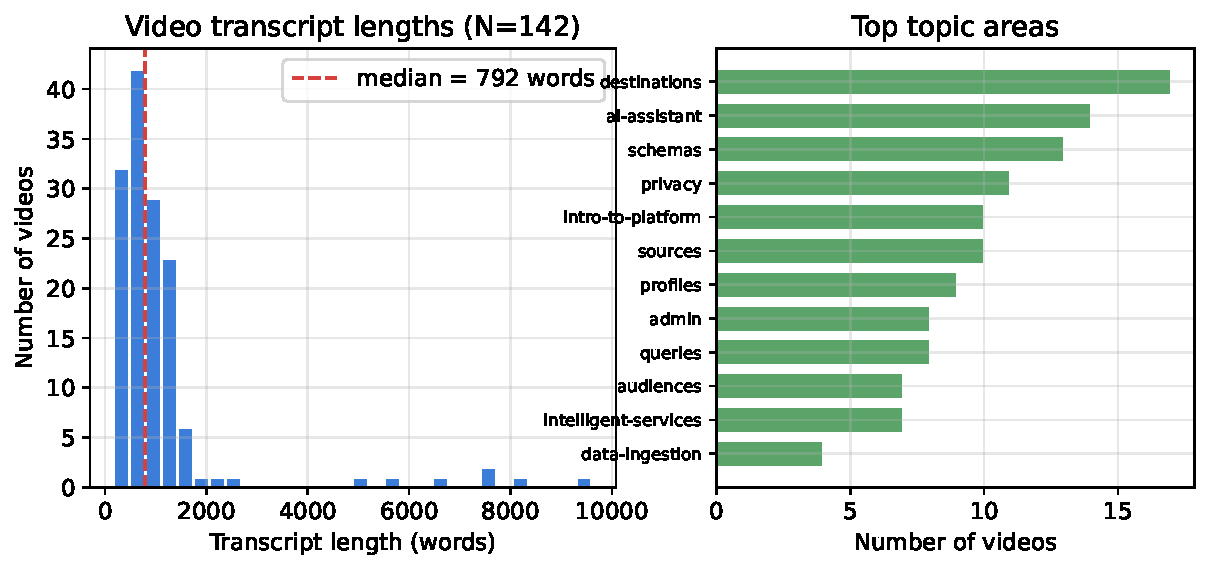
\includegraphics[width=\linewidth]{fig_transcript_lengths}
  \caption{Video-tutorial transcript corpus ($N=142$). Left: distribution of transcript
  length in words (median $\approx 792$, long right tail to $\sim 9.6$k words). Right:
  the twelve largest documentation topic areas. The corpus is AEP/AJO-centric and
  long-form, frequently exceeding standard $512$-token encoder budgets.}
  \label{fig:transcripts}
\end{figure*}

\subsection{Pairwise causal-classification datasets}

The central training signal is a \emph{directional pairwise} format: each row carries
\texttt{text\_1}, \texttt{text\_2}, and a binary \texttt{label}, where $\texttt{label}=1$
means \emph{\texttt{text\_1} causally precedes / enables \texttt{text\_2}}. The richer,
tiered variants additionally carry \texttt{tier\_1}, \texttt{tier\_2} (a curriculum-level
index), \texttt{sub\_1}, \texttt{sub\_2} (sub-chapter codes), and source URLs. We survey
the six datasets referenced as primary in the project context; their split sizes and
label balance are shown in Table~\ref{tab:datasets} and
Figures~\ref{fig:sizes}--\ref{fig:balance}.

\begin{table}[t]
  \centering
  \small
  \caption{Primary pairwise causal-classification datasets. Sizes are exact line counts;
  ``\%\,label\,1'' is the fraction of \emph{precedes} pairs in train; ``med.\ len.'' is the
  median word count of \texttt{text\_1}; ``tier'' marks datasets carrying tier metadata.
  Every dataset is essentially perfectly balanced by construction (forward/reverse pairs).}
  \label{tab:datasets}
  \begin{tabular}{lrrrcrc}
    \toprule
    Dataset & Train & Val & Test & \%\,lbl1 & med.\ len. & tier \\
    \midrule
    \texttt{aep\_causal\_cls34}    & 110{,}775 & 6{,}004  & 6{,}004  & 50.3 & 103 & \checkmark \\
    \texttt{hard\_neg\_sem}        & 261{,}210 & 14{,}736 & 6{,}004  & 50.3 & 103 & \checkmark \\
    \texttt{ajo\_doc\_not\_t1}     & 88{,}000  & 11{,}200 & 11{,}200 & 50.0 & 208 & \checkmark \\
    \texttt{new\_aep\_wf\_scrap}   & 13{,}904  & 1{,}676  & 1{,}548  & 50.0 & 44  & \\
    \texttt{workflowllm\_m2}       & 210{,}775 & 6{,}004  & 6{,}004  & 50.0 & 37  & \\
    \texttt{ajo\_newstyle}         & 20{,}897  & 2{,}612  & 2{,}613  & 50.0 & 95  & \\
    \bottomrule
  \end{tabular}
\end{table}

\paragraph{Label balance.} Because every dataset is built by emitting each ordered pair
in both directions ($\text{forward}\!\to\!1$, $\text{reverse}\!\to\!0$), the label
distribution is essentially exactly $50/50$ in every split
(Figure~\ref{fig:balance}). This is a deliberate and important property: it removes the
class-prior shortcut, forcing a model to learn \emph{directional asymmetry} rather than a
topical or frequency cue. It also means accuracy is directly interpretable against a
$50\%$ random floor, and that the genuine difficulty lives entirely in the
\emph{direction}, not in the marginal.

\paragraph{Scale and granularity.} Sizes span two orders of magnitude, from the
$\sim$17k-pair \texttt{new\_aep\_wf\_scrap} to the $\sim$282k-pair
\texttt{hard\_neg\_semantic} (Figure~\ref{fig:sizes}). Text granularity varies just as
widely: the workflow/phase datasets are short ($37$--$44$ word medians, single
action steps), whereas the conceptual document datasets are paragraph-scale
($103$--$208$ word medians). The \texttt{hard\_neg\_semantic} variant augments
\texttt{aep\_causal\_cls34} with semantically similar but causally unrelated distractors
(an explicit \texttt{hard\_neg} flag), roughly $2.4\times$ the base training size, to push
the model past lexical-overlap heuristics toward genuine causal discrimination.

\begin{figure}[t]
  \centering
  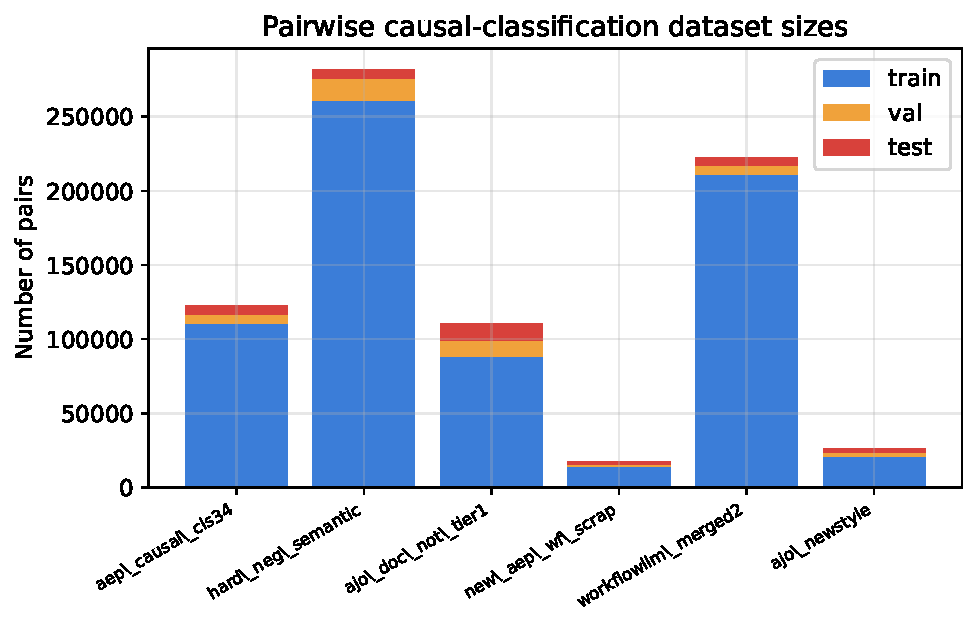
\includegraphics[width=\linewidth]{fig_dataset_sizes}
  \caption{Train/val/test sizes of the six primary pairwise datasets (stacked, exact line
  counts). Scale ranges from $\sim$17k to $\sim$282k pairs.}
  \label{fig:sizes}
\end{figure}

\begin{figure}[t]
  \centering
  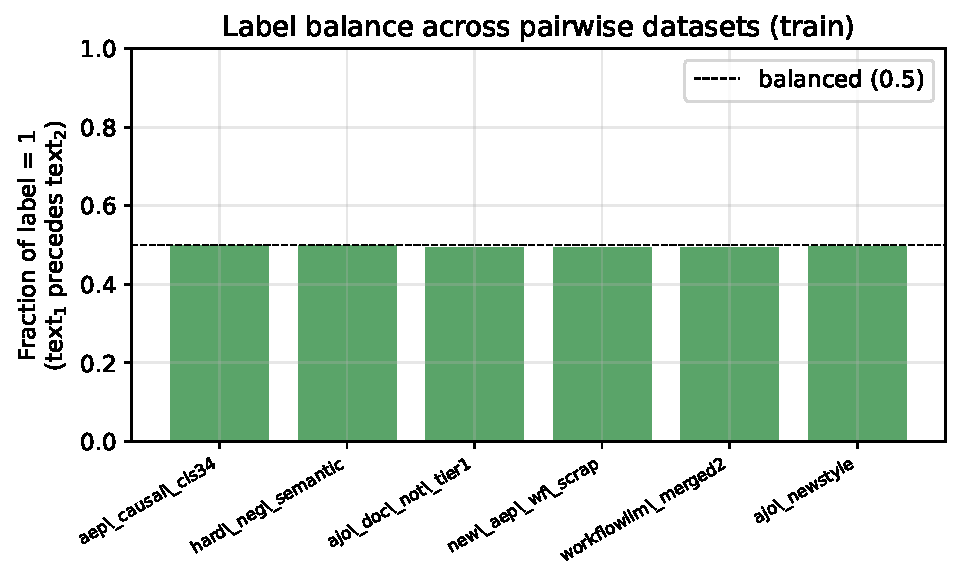
\includegraphics[width=\linewidth]{fig_label_balance}
  \caption{Label balance (fraction of $\texttt{label}=1$ ``precedes'' pairs, train split).
  Forward/reverse pair construction yields a $\approx 50/50$ split everywhere, eliminating
  the class-prior shortcut.}
  \label{fig:balance}
\end{figure}

\subsection{The tier system and the cross-tier gap}

The tiered AEP datasets attach to each text a \emph{tier} index ($\mathrm{T}1$--$\mathrm{T}15$)
derived from a fixed sub-chapter$\to$tier mapping (\texttt{directional\_manifest.json}). The
tier is a coarse position in the AEP learning curriculum: low tiers are foundational
(schemas, ingestion), high tiers are downstream (activation, journeys). The tier gap
$\lvert \texttt{tier\_1} - \texttt{tier\_2} \rvert$ thus measures how conceptually far
apart the two texts are.

The gap distribution is the single most consequential property of these datasets
(Figure~\ref{fig:tiergap}). For \texttt{aep\_causal\_cls34} and
\texttt{hard\_neg\_semantic}, \emph{no} training pair has gap $0$: both texts always come
from \emph{different} tiers, and the gap is broadly spread (modes at $1$--$4$, a long tail
out to $14$), with adjacent-tier pairs (gap $1$) being only $\sim$$13.5\%$ of the data.
These datasets therefore teach \emph{cross-tier} precedence over a wide conceptual span.
In sharp contrast, \texttt{ajo\_doc\_not\_tier1} is built \emph{within} documents, so its
pairs are confined to gap $0$/$1$ (same or immediately adjacent tier). The two regimes are
complementary --- broad cross-tier supervision versus fine intra-document supervision ---
but they are \emph{not interchangeable}, and a model trained on one is evaluated
implicitly on the other.

\begin{figure*}[t]
  \centering
  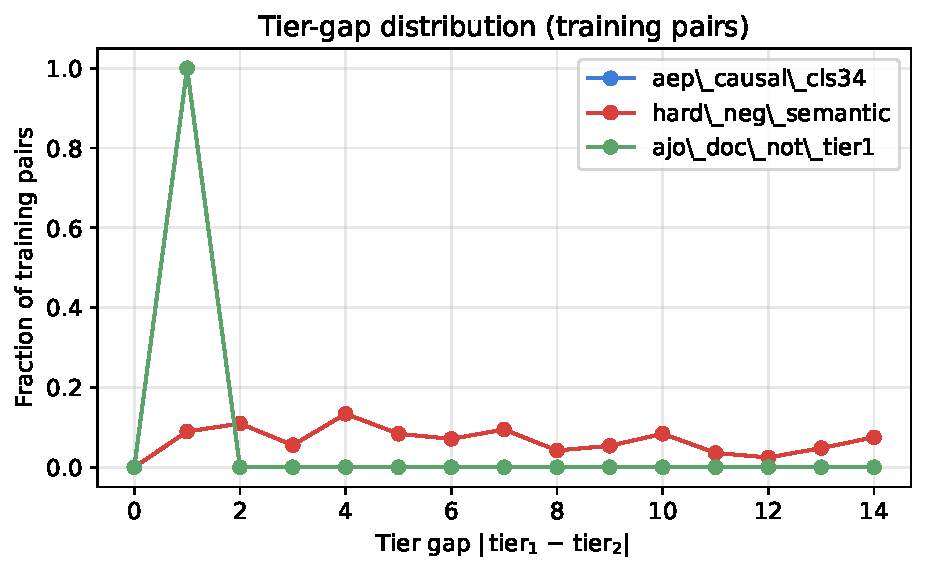
\includegraphics[width=\linewidth]{fig_tier_gap_dist}
  \caption{Tier-gap $\lvert \texttt{tier\_1}-\texttt{tier\_2}\rvert$ distribution over
  training pairs. The cross-document datasets (\texttt{aep\_causal\_cls34},
  \texttt{hard\_neg\_semantic}) span gaps $1$--$14$ and contain \emph{no} same-tier pairs,
  whereas \texttt{ajo\_doc\_not\_tier1} is confined to gaps $0$/$1$. This complementarity
  is the structural source of train/test distribution shift.}
  \label{fig:tiergap}
\end{figure*}

\subsection{Adjacency / \texttt{MAX\_GAP} labeling and its distribution shift}

The workflow datasets reveal a second, finer adjacency constraint --- imposed not at the
tier level but at the \emph{step} level within a single document. The deterministic
extractor builds ordered pairs only between phases at most \texttt{MAX\_GAP} positions
apart: \texttt{MAX\_GAP}$=2$ (consecutive $+$ skip-one) for
\texttt{new\_aep\_workflow\_scrap}, and gap$\le 4$ (capped at $60$ pairs per document) for
the AJO sentence-level builder. Empirically, $100\%$ of \texttt{new\_aep\_workflow\_scrap}
training pairs have step gap $1$ ($56.5\%$) or $2$ ($43.5\%$) --- the model \emph{never}
sees a far-apart pair during training. Splits are document-level $80/10/10$ (seed $42$)
with no URL leakage across splits, and forward/reverse pairs keep labels balanced.

This windowing is well-intentioned --- it kills the topic shortcut and keeps pairs locally
coherent --- but it creates a hard \textbf{train/eval distribution shift}. At evaluation
time the orderer must score \emph{all} $\binom{n}{2}$ pairs of an $n$-step workflow,
including the far-apart (gap $\gg \texttt{MAX\_GAP}$) pairs that never appeared in
training. The independent-embedding bi-encoder, which excels on the adjacent in-distribution
pairs, degrades on these off-distribution long-range pairs; the cross-encoder's joint
cross-attention generalizes further, which is consistent with the repository's finding that
the DeBERTa-v3-large cross-encoder reaches $21/30$ correct workflow orderings on
\texttt{new\_ajo\_workflows} versus a bi-encoder's $0/30$. A second confound compounds it:
the format forces a \emph{total order} (every pair gets a direction) with \emph{no neutral
class}, yet real procedures are partial orders containing genuinely parallel/independent
steps. Forcing a chain over noisy, occasionally cyclic pairwise scores makes errors
compound. These two artifacts --- adjacency-only supervision and the total-order assumption
--- are the structural roots of the end-to-end ordering failure.

\subsection{Workflow-ordering and follow-up evaluation sets}

\paragraph{Workflow ordering.} The downstream ordering target
\texttt{ajo\_orchestrated\_workflows\_flat.json} contains $30$ orchestrated AJO
workflows, each \emph{uniformly} $3$ steps (\texttt{t1}/\texttt{t2}/\texttt{t3}), written
in a clean LLM-orchestrated style (e.g.\ select abandoned-cart profiles
$\to$ enrich with cart data $\to$ send personalized email). Four auxiliary
\texttt{aep\_3step\_workflows*} sets ($10$ workflows each; \emph{simple}, \emph{specific},
and \emph{transcript} stylistic variants) provide additional $3$-step probes. The small,
short, clean nature of these eval targets contrasts sharply with the long, noisy training
transcripts --- another axis of distribution shift between train and evaluation.

\paragraph{Follow-up reranking.} The follow-up dataset
(\texttt{prod\_jan\_feb\_26-aep-ajo\_follow-up-queries.json}) contains $334$ real AEP/AJO
anchor questions, each paired with \emph{exactly} $10$ candidate follow-up queries
(Figure~\ref{fig:followup}, left). Anchor questions are short --- mean $\approx 17.5$
words. The uniform $10$-candidate structure makes this a clean fixed-list reranking
benchmark (ideal for MRR / Recall@$k$), but it carries no gold relevance labels in the
raw file, so supervision or evaluation requires an external relevance signal.

\begin{figure}[t]
  \centering
  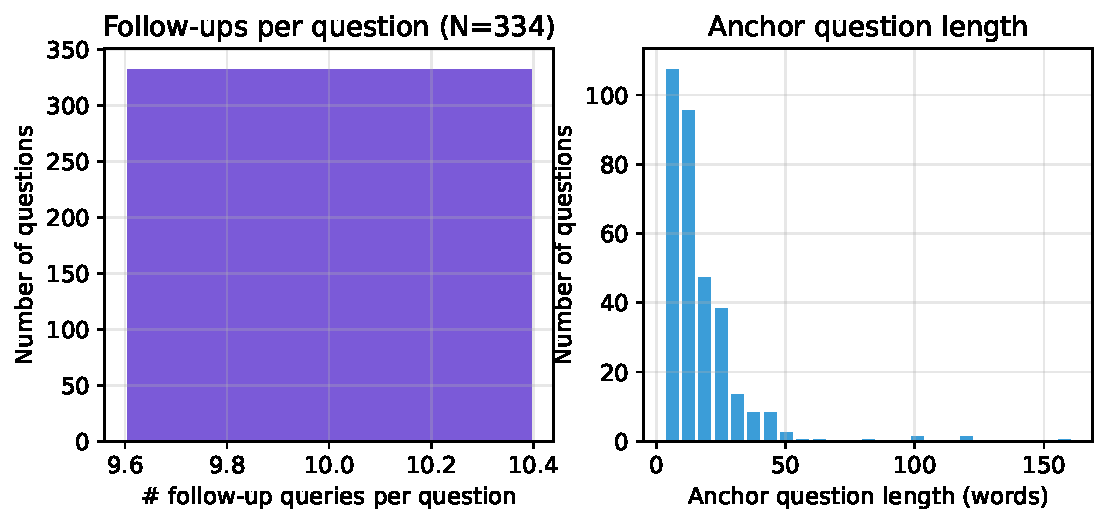
\includegraphics[width=\linewidth]{fig_followup_counts}
  \caption{Follow-up reranking set ($N=334$ anchor questions). Left: each question has
  exactly $10$ candidate follow-ups (a fixed-list reranking setup). Right: anchor-question
  length distribution (mean $\approx 17.5$ words).}
  \label{fig:followup}
\end{figure}

\subsection{Implications for modeling}

Four data properties should drive modeling decisions. \textbf{(1) Direction is the whole
task.} The enforced $50/50$ balance removes priors, so every gain must come from modeling
the antisymmetry $P(\text{A}\!\prec\!\text{B}) \neq P(\text{B}\!\prec\!\text{A})$ ---
motivating directional fusion, asymmetric scoring, or order-aware objectives over plain
symmetric similarity. \textbf{(2) Adjacency-only / \texttt{MAX\_GAP} supervision under-fits
long-range ordering.} Training only on gap-$\le$$2$/$4$ pairs but evaluating on all pairs
is the dominant distribution shift; closing it argues for training on the full transitive
closure within a document (far-apart pairs included), which also explains why the
cross-attention cross-encoder generalizes better than independent bi-encoder embeddings.
\textbf{(3) The total-order assumption is wrong.} With no neutral/abstain class, parallel
steps are mislabeled and forced into a chain; adding a neutral class and aggregating with a
cycle-tolerant ranker (Bradley--Terry / minimum-feedback-arc-set / Kemeny) rather than a
naive topological sort should reduce compounded ordering errors. \textbf{(4) Length and
style mismatch.} Long-form transcripts ($\sim$792-word median, $9.6$k-word tail) exceed
$512$-token budgets and differ stylistically from the short, clean $3$-step eval workflows;
this favors models that avoid truncating both texts into one shared budget and motivates
explicit train/eval style-gap mitigation. The tiered/hard-negative datasets and the fixed
$10$-candidate follow-up set are well-suited respectively to curriculum-style training and
to clean MRR-based reranking evaluation.

\section{Synthesis: A Recommended Sub-1B Causal Embedding System}

This section pulls the survey together into a single, concrete design for the \aep/\ajo
setting, ranked by return on investment (impact divided by cost/risk), under the
sub-1B-parameter constraint. The guiding empirical fact---established in the data and
baselines (Section~10) and across the surveyed literature---is that \emph{pairwise
accuracy does not equal ordering quality}: the DeBERTa-v3 cross-encoder is already strong
on pairs (21/30) yet the end-to-end ordering is 0/30. The dominant losses are therefore in
\textbf{aggregation} and \textbf{data}, not in the pairwise model.

\subsection{The three sub-problems}
Any system for this task decomposes into:
\begin{enumerate}[leftmargin=1.4em,itemsep=0.1em]
  \item \textbf{Pairwise scorer} --- ``does step $A$ causally precede $B$?'' (the
  cross-encoder is strong here).
  \item \textbf{Data} --- which pairs/labels the scorer is trained on (currently
  adjacent-only within a document, forced total order, no \textsc{neutral}).
  \item \textbf{Aggregation} --- turning $O(n^2)$ noisy pairwise scores into one global
  order (currently naive topological sort, which cannot survive a single cycle).
\end{enumerate}
The cheapest, highest-impact wins are in (2) and (3) and require \emph{no new model}; the
reasoning/RL work raises the ceiling on top of them.

\subsection{Tier 1 --- highest ROI, no new model}
\paragraph{Robust rank aggregation (the single biggest win).}
Replace topological sort with \emph{calibrated, confidence-weighted minimum-feedback-arc-set
(MFAS) / Kemeny ``minimum-violations'' ordering} (Section~7). Edges are weighted by the
log-odds of the pairwise $P(\text{precedes})$; solve with the linear-time Eades--Lin--Smyth
heuristic (\texttt{python-igraph}'s \texttt{feedback\_arc\_set}; note NetworkX has no FAS
routine) or an exact ILP since workflows are tiny (3--12 steps). Unlike topological sort,
MFAS/Kemeny degrade gracefully under cycles. Our reference implementation provides this and
demonstrates it on the 30 \ajo\ workflows.

\paragraph{Calibrate before aggregating.}
Temperature-scale the cross-encoder logits on the validation set (Section~7). Calibration
preserves arg-max (so pairwise accuracy is unchanged) but makes confidence-weighted edges,
thresholds, and abstention behave correctly.

\paragraph{Train on the full within-document transitive closure.}
Positional precedence is transitive, so every $i<j$ pair within a document is a valid label,
yet the data emits only adjacent ($\text{gap}\le 2/4$) pairs while evaluation requires
ordering \emph{all} pairs of a workflow. Dropping \texttt{MAX\_GAP} closes this distribution
shift (Section~10); adding pairwise distance as an auxiliary target sharpens long-range
judgments.

\paragraph{Evaluate as a partial order.}
Report tie-aware Kendall-$\tau$ ($\tau_b/\tau_c$) and precedence-pair precision/recall, not
just exact-permutation accuracy (Section~7). Real workflows contain parallel steps; exact
matching hides genuine progress and provides no usable training/RL signal.

\subsection{Tier 2 --- the reasoning model, on the backbone that wins}
Naive chain-of-thought \emph{degrades} pointwise rerankers (Section~6), so for the pointwise
causal scorer we prefer \emph{internalized / ``think-free'' reasoning}.
\paragraph{Distill causal rationales into the cross-encoder (recommended primary).}
Keep the DeBERTa-v3 CE; add an auxiliary rationale objective in which a teacher LLM writes a
short causal explanation per pair (reject-sampled to agree with the gold label), and the CE
learns to both predict direction and match the rationale representation. This extends the
repo's existing \texttt{ReasoningClassifier} (frozen-encoder explanation embedding +
cosine loss), adds \emph{zero} inference latency, and is strongly supported by
\emph{Distilling Step-by-Step} and TFRank-style think-free training (Section~6).
\paragraph{Sub-1B generative reasoner (ceiling track).}
In parallel, train a $\sim$0.6B generative model (e.g.\ Qwen3-0.6B) as a pointwise
precedence scorer with a think-mode switch---reasons during training, runs think-free at
inference, emits \textsc{precedes/follows/neutral} plus a graded score. TFRank ships a 0.6B
checkpoint as existence proof. Pick the winner of the two tracks on the latency/accuracy
curve.
\paragraph{Bootstrap rationales and a \textsc{neutral} class.}
Generate teacher CoT per pair, reject-sample to the gold label (STaR/RFT/COLLATE-style),
optionally VeriCoT-validate for consistency; and \emph{mine \textsc{neutral} pairs}
(cross-document unrelated steps; same-document steps under sibling/parallel headings whose
order is swap-invariant). \textsc{neutral} lets the orderer emit antichains (a DAG) instead
of hallucinating edges between parallel steps.

\subsection{Tier 3 --- push the ceiling}
\paragraph{Ordering-reward GRPO polish.}
After distillation/SFT, a \emph{short} GRPO run with a reward of format + pairwise direction
correctness + Kendall-$\tau$/NDCG against gold order on sampled whole workflows (REARANK /
Rank-GRPO precedent). Use Dr.GRPO/DAPO fixes for length bias and entropy collapse; LoRA
first. The literature is consistent that sub-1B models should be \emph{distilled first, then
RL-polished}, not RL-trained from scratch (Section~6).
\paragraph{Listwise / global ordering.}
Longer term, move from pairwise-then-aggregate toward a global objective---ListMLE /
Plackett--Luce NLL, a pointer/seq2seq orderer, or a Set-Encoder-style listwise
cross-encoder---to stop per-pair errors from compounding (Section~7).
\paragraph{Asymmetric-geometry retriever.}
For \emph{scalable} first-stage directional retrieval (where a cross-encoder is too slow),
an order/box/hyperbolic head or a dual ``cause''/``effect'' projection (Section~5) provides a
genuinely asymmetric score at embedding speed; keep the cross-encoder as the precise
second stage.

\subsection{The recommended pipeline}
\begin{quote}\small\ttfamily
Stage 1  Retriever (existing BGE-large bi-encoder; optional asymmetric head) \\
Stage 2  Causal reasoner (PRIMARY: DeBERTa-v3 CE + distilled rationale head; \\
\phantom{Stage 2  }TRACK B: Qwen3-0.6B think-free generative) \\
\phantom{Stage 2  }$\rightarrow$ calibrated P(precedes), 3-way incl. NEUTRAL \\
Stage 3  Orderer = weighted MFAS / Kemeny over log-odds edges; \\
\phantom{Stage 3  }low-confidence pairs $\rightarrow$ antichains (DAG) \\
Stage 4  Verifier (VeriCoT-style) breaks residual cycles \\
Eval     tie-aware Kendall-$\tau$ + precedence P/R; later GRPO $\tau$-reward
\end{quote}
\textbf{Training order:} distill rationales $\rightarrow$ SFT CE/0.6B $\rightarrow$ optional
GRPO $\tau$-reward; data upgraded to full transitive closure $+$ \textsc{neutral};
aggregation upgraded to calibrated Kemeny.

\subsection{First-week plan (most gain needs no training)}
(1) Swap topological sort for calibrated weighted-MFAS and re-score the existing DeBERTa-CE
outputs on the milan/\ajo\ sets---this alone should move 0/30 sharply. (2) Add Kendall-$\tau$
+ precedence-P/R to the eval harness. (3) Drop \texttt{MAX\_GAP}, regenerate
full-transitive-closure pairs, retrain the CE. (4) Measure, \emph{then} invest in the
reasoning track. The reference implementation released with this survey covers steps (1)
and (2) out of the box.

\subsection{Empirical validation (reference implementation)}
The reference implementation released with this survey (\texttt{implementation/}) lets us
test the Tier-1 claims directly. Two findings stand out. First, on a controlled
decent-but-noisy, cyclic pairwise signal ($\sim$0.80 pairwise accuracy, presentation
shuffled to remove input-order leakage), robust aggregation recovers roughly
$3\times$ the perfect-match rate of naive topological sort, as pure post-processing with no
model change:

\begin{table}[h]
\centering\footnotesize
\begin{tabular}{lccc}
\toprule
Aggregator & PMR & Kendall $\tau_b$ & Prec.\ F1 \\
\midrule
Naive topo-sort       & 0.104 & 0.243 & 0.622 \\
Bradley--Terry        & 0.265 & 0.806 & 0.903 \\
MFAS (weighted)       & \textbf{0.317} & \textbf{0.816} & \textbf{0.908} \\
Kemeny (exact, small) & \textbf{0.317} & \textbf{0.816} & \textbf{0.908} \\
\bottomrule
\end{tabular}
\caption{Ordering quality from the same pairwise scores under different aggregators
(controlled noisy/cyclic regime). Robust aggregation $\approx 3\times$ the perfect-match
rate (PMR) of topological sort.}
\end{table}

Second---and crucially---aggregation only helps when the pairwise signal is
\emph{decent}. Wiring in the project's \emph{real} scored workflows confirms the
diagnosis: the bi-encoder's pairwise scores agree with gold precedence only
$\sim$41\% of the time (worse than chance), so \emph{no} aggregator can order them---this
is the documented 0/30. The cross-encoder scores are $\sim$96\% accurate, and \emph{every}
aggregator then orders all evaluated workflows correctly. The practical implication is
twofold: (i) the cross-encoder is the right backbone (it makes the signal aggregable), and
(ii) robust aggregation is the lever that converts that signal into correct global orders
once it is decent-but-noisy. The bi-encoder's failure is not an aggregation problem to be
post-processed away---it is a signal problem requiring the better pairwise model.

\subsection{Honest expectation-setting}
Causal \emph{direction} is hard even for frontier models, and supervised systems cap well
below ceiling (Section~4). Reasoning + distillation is precisely the lever shown to help,
but no orderer will be perfect. The realistic, defensible win is to \emph{fix aggregation
and data (Tier 1) to convert the existing pairwise strength into a much higher ordering
score}, then use distilled reasoning and a $\tau$-reward GRPO polish (Tiers 2--3) to push
further.

\section{Conclusion}

We set out to answer whether one can build a \emph{causal embedding model}---a
representation and scoring function that captures directional precedence rather than
topical similarity---capable of judging causal direction, reranking follow-up questions,
and sorting \aep/\ajo\ workflow steps into order. Surveying causal foundations, dense
retrieval, causal reasoning from text, asymmetric/order-structured geometry, reasoning
rerankers and RL, sentence-ordering and rank aggregation, follow-up/conversational
retrieval, and procedural-workflow understanding, three conclusions stand out.

\paragraph{1. ``Causal'' here is mostly structural precedence.} The task lives largely on
Pearl's associational/structural rung---ordering steps by enablement within procedural
text---rather than on intervention or counterfactuals. This is liberating: it can be
attacked with directional supervised learning and reasoning, without the full apparatus
of causal discovery. It is also a caution against over-claiming ``causality.''

\paragraph{2. Symmetry is the architectural mismatch; the cross-encoder and asymmetric
geometries are the answers.} Cosine-similarity embeddings cannot represent direction by
construction. Cross-encoders recover it through joint cross-attention (and win on
ordering despite losing on pairwise classification), while order/box/Gaussian/hyperbolic
embeddings and dual cause/effect projections offer asymmetric scoring at embedding speed
for scalable first-stage retrieval.

\paragraph{3. The ordering bottleneck is aggregation and data, not the pairwise model.}
The most actionable finding is that a 21/30 pairwise model collapses to 0/30 full
orderings under naive topological sort. Replacing it with calibrated, confidence-weighted
minimum-feedback-arc-set / Kemeny aggregation, training on the full within-document
transitive closure (not just adjacent pairs), adding a \textsc{neutral} class for
partial orders, and evaluating with tie-aware Kendall-$\tau$ together address the failure
\emph{before} any new model is trained.

On top of this foundation, the survey points to a sub-1B reasoning track---think-free
rationale distillation into the cross-encoder as the safe primary, a 0.6B generative
reasoner as the ceiling, and a short ordering-reward GRPO polish---as the way to push
beyond what aggregation fixes alone can buy. The accompanying reference implementation
makes the Tier-1 wins (robust aggregation, calibration, partial-order metrics, follow-up
reranking) immediately runnable.

\paragraph{Limitations and future work.} Causal direction remains hard even for frontier
models; gold reasoning traces must be bootstrapped; and the \textsc{neutral}/partial-order
labels need mining. Promising directions include listwise global ordering to eliminate
error compounding, learned asymmetric retrieval heads benchmarked against the cross-encoder,
and a dedicated directional/causal evaluation suite---absent from current embedding
leaderboards---to measure progress on precisely the capability this project needs.


\bibliographystyle{plainnat}
\bibliography{refs}

\end{document}
